\documentclass[12pt,letterpaper]{article}
\usepackage{times}
\usepackage[utf8]{inputenc}
\usepackage[spanish]{babel}
\usepackage[authoryear]{natbib}
\usepackage{amsthm,amsmath,amsfonts,amssymb}
\usepackage[doublespacing]{setspace}
\usepackage{graphicx}
\usepackage{tabularx}
\usepackage{caption}
\usepackage{subcaption}
\usepackage{arydshln}
\usepackage{lscape}
\usepackage{pdflscape}
\usepackage{hyperref}
\usepackage{cleveref}
\usepackage[top=3cm, bottom=3cm, left=3cm, right=3cm]{geometry}


%\usepackage{setspace}
%\singlespacing
%\onehalfspacing
%\doublespacing
%\setstretch{1.1}

\title{Tipo de Cambio Real de Equilibrio de Bolivia} 

%\author{Hugo Pablo Rocha Portugal \and Paola Cecilia Yujra Tonconi}
\author{10195}

\date{\today}

\begin{document} 

\maketitle 

\begin{abstract}
\singlespacing

En el presente documento está contextualizado alrededor de la discusión del paradigma de crecimiento económico basado en la competitividad externa. Para contrastar esta idea, se analizan las políticas cambiarias bolivianas que buscaron este objetivo. Para dicho efecto, se plantea estudiar el desempeño de las mismas con respecto a la senda de equilibrio del tipo de cambio real. El análisis permite no solo determinar la relevancia y compatibilidad de estos métodos con las características particulares de la economía revisada, sino también propone elementos importantes para poder construir una medida más relevante y apropiada de equilibrio. En el documento se encuentra que el tipo de cambio real no es una medida de competitividad externa para las exportaciones bolivianas aunque tienen un efecto particular en las importaciones. Por otro lado, se propone que la política cambiaria de tipo de cambio nominal no es la mejor manera de estimular cambios en el TCR. Finalmente, se encuentra el conjunto de fundamentos relacionados con la dinámica de la serie en cuestión.
\\
\\
\bigskip
Palabras clave: Estimación, BEER, DEER, Tipo de Cambio Real, Economía abierta \\
Clasificación JEL: E500, F140, C510

\end{abstract}

\newpage

\section{Introducción}

%A pesar que la estructura económica de Bolivia ha evolucionado, se debe destacar que existen persistentes características que determinan la identidad de la misma. Estudios que las particularizan están diseminados a través de la memoria académica del país, de entre los cuales muy pocos lograron trascender el ámbito local como testimonio elocuente del funcionamiento de la economía boliviana y muchos de autoría foránea no siempre consiguen plasmar comprehensiblemente la realidad del caso. Asimismo, estos documentos son selectivos en los rasgos característicos de la economía, esta selectividad abusa del proceso de pesquisa de la disciplina económica que utiliza supuestos y simplificaciones fuertes obteniendo conclusiones altamente cuestionables. En este documento no se pretende discutir las consecuencias de esta práctica pero se pretende ofrecer un análisis que amalgama las practicas comunes de la economía empírica con el contraste de la observación crítica de la historia económica.

%En este sentido, de entre la evidencia que destaca la existencia de ciclos en la economía boliviana se debe rescatar que el registro del último ciclo, tomando como punto de referencia la actualidad, se data su inicio hace más de 40 años. Sin embargo, incluso siendo este periodo perteneciente al periodo moderno de la economía no se tiene una colección de datos completa, estando disponible menos del 75\% de ellos. Por lo tanto, se plantea revisar históricamente hitos importantes que determinaron comportamientos persistentes y quiebres estructurales de los momentos en los que no se tienen datos y realizar un análisis empírico a través de aquellos periodos con disponibilidad de información cuantitativa.

Tras la devastadora hiperinflación que Bolivia sufrió durante la primera mitad de la década de los ochenta, la economía local se restituyó habiéndose logrado una solución satisfactoria, unificando los mercados cambiarios, que puso fin a dicha patología en precios y poniéndole un alto a la depreciación descontrolada de la moneda que dio paso a la creación de una nueva. Sin embargo, características como contrabando, informalidad, corrupción, pobreza y dolarización fueron cada vez más comunes en las descripciones de la economía durante el posterior periodo de estabilización. La delicadeza de la situación estaba determinada por un proceso de insipiente crecimiento debido a su economía primaria e informal combinada con la dependencia de las importaciones y el régimen cambiario \emph{crawling peg}. Las constantes devaluaciones de la moneda local generaron una alta dependencia al dólar americano y limitaron la efectividad de la política monetaria. Los bienes importados tenían precios en bolivianos cada vez mayores por el costo elevado de importación y la constante depreciación de la moneda local, haciendo que la preferencia por moneda se traslade a la divisa estadounidense. Este hecho combinado con los bajos niveles de remuneración y precariedad del mercado laboral profundizaron la informalidad y el contrabando, el primero como alternativa de fuentes de ingreso y el segundo como fuente de abastecimiento barato. Esta última relación generó un círculo de complementariedad entre ellos. 

Al mismo tiempo, las condiciones particulares por las que la economía pasaba no permitieron cambiar su matriz productiva al paradigma industrial a diferencia de sus vecinos regionales que ya habían logrado incurrir en este camino décadas atrás; la explotación de materias primas para exportación aún constituía el factor de crecimiento característico de la economía boliviana, así como lo fue desde épocas coloniales y durante toda la república. Por un lado, los costos de producción eran muy elevados desde el punto de vista capital pues gran parte de esa inversión debería ser importada, limitando la llegada de nuevas tecnologías. Este hecho generó la búsqueda de competitividad en precios de las industrias que sacrificaron productividad y calidad, a través de salarios bajos y poca reinversión en capital, en un esquema de debilidad institucional que no velaba por el bienestar social de la sociedad. Como consecuencia de ello, el crecimiento económico en la década de los noventa que se constituye en la parte de estabilización y crecimiento del nuevo paradigma económico después de la hiperinflación fue limitado y caracterizado por la inestabilidad política. Sin embargo, a mediados de la década de 2000's, el incremento de precios de materias primas sumado a la nacionalización de hidrocarburos se constituyeron en elementos claves para que Bolivia presente mejorías en sus indicadores macroeconómicos y sociales.

%Exito económico
El éxito del país en materia económica es sobresaliente desde 2004-2005 hasta la 2014. Efectivamente, el país pasó de ser uno de los más pobres del subcontinente a tener el crecimiento económico más importante de la región. Al mismo tiempo, consiguió recaudar elevados niveles de Reservas Internacionales Netas (RIN), reducir los niveles de pobreza y desigualdad, des-dolarizar su economía, reducir los niveles de deuda y mantener niveles controlados de inflación. Incluso cuando los términos de intercambio no le favorecieron, a partir de 2014, Bolivia demostró una gran capacidad de resiliencia aplicando políticas macro prudenciales y contra-cíclicas. Ante todos estos logros queda preguntarse cuales fueron los factores más importantes que contribuyeron a su consecución.

%Sector externo
Sin lugar a dudas, el desempeño de la balanza comercial de este periodo de expansión, destacado previamente, se constituye en el influjo de divisas y riqueza más importante desde finales de la década de los setenta. A partir de 2004 y consolidándose a finales de 2005, las exportaciones de hidrocarburos presentaron valores elevados los cuales se incrementaron significativamente periodo tras periodo. La nacionalización de 2006 fue una de las políticas nacionales más importantes pues permitió que el país capte, utilice y distribuya estas ganancias siendo que previo a esta medida quien se quedaba con la mayoría de las utilidades eran las empresas trans-nacionales que operaban la exploración y explotación de recursos naturales en Bolivia. Por estas razones, este fenómeno está altamente correlacionado con el citado éxito económico. En este sentido, no es casualidad que la meta de las pasadas autoridades políticas y económicas del país haya estado orientada a procurar la bonanza de comercio internacional basando sus esperanzas en políticas dirigidas al desempeño del sector extractivo.

En este periodo de boom, los impuestos directos a los hidrocarburos permitieron al gobierno central emprender políticas públicas importantes como la implementación de bonos sociales dirigidos principalmente a niños, madres en gestación y adultos mayores, los cuales constituyen la población más vulnerable del país. Asimismo, dichos influjos permitieron el incremento de las RIN y gasto e inversión pública ejecutados a través del gobierno central así como por los gobiernos departamentales y municipales. Los proyectos públicos con mayor notoriedad financiados por estos recursos fueron las Empresas Públicas Nacionales Estratégicas (EPNE), obras en la red de caminos y construcción de infraestructura. Al mismo tiempo, esta inyección de circulante en la economía, primero a través del gasto público y después por la política monetaria, permitió a su vez el fomento del gasto privado e inversión privada magnificando los resultados, siendo, en los últimos años, el incremento de circulante en el sistema financiero orientado en crédito a la vivienda social y al sector productivo la principal política monetaria expansiva posterior a 2014. 

Acerca del tema de políticas cambiarias y monetarias se puede destacar que después del periodo de estabilización, la subida de precios internacionales de materias primas a partir de 2004-2005 trajo consigo, además del éxito exportador, inflación en la economía la cual pudo ser contenida gracias al respaldo y confianza de la población en las RIN recién acumuladas. La política cambiaria de continuas depreciaciones que se llevaban a cabo hasta entonces cambió de dirección hacia la apreciación del boliviano y una política monetaria contractiva. Estas medidas contribuyeron, junto a otras, a la des-dolarización financiera de la economía. Habiéndose contenido las presiones inflacionarias, la crisis financiera internacional generó la demanda de dólares en la economía generando presiones de devaluación que fueron contenidas con la estabilidad cambiaria. Tras este evento, el repunte de los precios internacionales y otras crisis externas implicaron la reaparición de presiones inflacionarias que fueron combatidas apreciando la moneda por un último periodo. Finalmente, a partir de 2012 se ha estabilizado el movimiento cambiario hasta la actualidad. En resumen, el Banco Central de Bolivia aduce que la estabilidad cambiaria actual ha permitido mitigar las presiones inflacionarias de origen externo, anclar las expectativas de los agentes económicos con respecto del valor del dólar y des-dolarizar financieramente la economía. Por otro lado, después de la caída de precios internacionales en 2014 el BCB procedió la ejecución anticíclica de la orientación de la política monetaria inyectando recursos en la economía

En contraste y para dar contexto a la política cambiaria en la etapa de boom, durante la década de los noventas y tras la estabilización post-hiperinflación, el crecimiento económico a través de exportaciones, des-dolarización, ejecución soberana de la política monetaria se constituyen en el santo grial perseguido por los hacedores de política bolivianos que a través de la devaluación cambiaria buscaron generar la suficiente competencia externa para lograr dicho cometido. Es decir, plantearon a la devaluación nominal como el instrumento para devaluar el tipo de cambio real (TCR) en la dirección que permita incrementar las exportaciones. Esto debido al paradigma económico, que se manejó e incluso aún se maneja, basado en que la competitividad de tipo de cambio fomentaría las exportaciones de recursos naturales y estos a su vez generarían utilidad económica y entrada de divisas, activos con los cuales se conseguiría la solución a todos los problemas inmediatos y acumulados de la economía nacional los cuales son reclamos de la sociedad boliviana. Bajo este concepto, es importante estudiar el periodo de apreciaciones nominales que permitió la consecución de los objetivos buscados con competitividad externa y éxito comercial internacional.

%TCR como nivel de competitividad
Debido a la importancia que las exportaciones tienen para la economía de Bolivia es pertinente estudiar aquellas variables económicas que las fomentan y los comovimientos que comparten. Si bien los términos de intercambio y la nacionalización de hidrocarburos sin lugar a duda beneficiaron al crecimiento, se deben identificar las políticas económicas que hayan logrado o podido haber logrado aprovechar el importante periodo de bonanza. En teoría, la más importante de ellas es la política cambiaria que podría haber definido el tipo de cambio real que teóricamente captura la competitividad de los productos bolivianos comparado con sus principales socios comerciales. Teóricamente, la depreciación de esta variable implicaría el abaratamiento de los bienes y servicios nacionales haciéndolos más atractivos para sus compradores internacionales, generando el incremento de las exportaciones.

%Estabilidad cambiaria y como el TCN determina al TCR
%Como ya ha sido adelantado, los hacedores de política fueron conscientes de la importancia del tipo de cambio real y de la bonanza en exportaciones. En efecto, el proceso cambiario de finales de los 80s hasta 2005 denominado \emph{crawling peg} se constituyó en la política cambiaria boliviana que tuvo como objetivo principal incrementar la competitividad nacional a través de constantes mini devaluaciones no anunciadas que, según el plan, permitirían mantener un tipo de cambio real consistente con un equilibrio en la balanza comercial. Sin embargo, a pesar del esfuerzo que implicó dicho régimen cambiario, no se logró el objetivo asumido sino hasta finales de su vigencia. De igual manera, llama la atención que el incremento de las exportaciones sucedió cuando el tipo de cambio real atravesó una fase de profunda apreciación implicando un hecho contrario a lo adelantado por la teoría.

%TCReq para saber cual es la mejor política cambiaria, cuanto cuesta mantener el tipo de cambio fijo y desalineamientos y como se mueve
En este marco, se propone estudiar el tipo de cambio real desde la perspectiva de su equilibrio. Esto permitiría encontrar el nivel de balance entre el denominado equilibrio interno y externo, es decir el tipo de cambio real que propiciaría la competitividad externa y condiciones internas de la economía para lograr crecimiento sostenible. Los valores observados del TCR y su variable calculados de equilibrio determinan el desalineamiento cambiario al que se puede atribuir el los déficits en balanza comercial y se constituirían en condiciones que limitarían el crecimiento de la economía interna. Al mismo tiempo, el análisis podría indicar cual es la mejor política que se podría haber aplicado y se puede aplicar en el futuro. Adicionalmente, la estimación de este equilibrio cambiario, otorgaría información sobre el set de variables que llegan a determinarlo a través de la política económica.

%Lo que se encuentra en el paper
En este sentido, se utilizan dos metodologías convencionales y complementarias para calcular el tipo de cambio real de equilibrio, las cuales son \emph{behavioral equilibrium exchange rate} BEER y \emph{desired equilibrium exchange rate} DEER. La primera aproximación se enfoca en establecer los determinantes que se espera tengan efectos persistentes y de mediano plazo en el tipo de cambio real. Esta metodología encuentra que el tipo de cambio real en tendencia siempre se mantiene bajo la senda de su equilibrio con leves desviaciones del mismo. La segunda metodología propone que los desalineamientos se encuentran antes de 2003 y después de 2013, momentos en los que los precios en materias primas no beneficiaron los términos de intercambio. El uso complementario de estas dos metodologías permiten entender, a través del primer modelo, cuales son las variables que afectan el movimiento del TCR y su correspondiente equilibrio y, mediante el segundo modelo, se puede observar cuál es el nivel de depreciación del tipo de cambio real que mejora los niveles de cuenta corriente. Sin embargo, a partir de un análisis más profundo, se encuentran las debilidades de estos métodos aplicados en el caso boliviano, y al mismo tiempo, estas consideraciones ayudan a entender mejor la economía boliviana y sus particularidad a través de las cuales se puede reconsiderar una mejor forma de medir el tipo de cambio real de equilibrio.

Este documento encuentra que la variable que explica los incrementos de exportaciones y balanza comercial no es la depreciación del tipo de cambio real; el éxito económico aparentemente depende de los términos de intercambio y en el caso específico por la consecuente nacionalización de hidrocarburos que permite que el gobierno perciba los beneficios derivados de la venta de los recursos explotados. El incremento de precios de hidrocarburos es independiente de las políticas bolivianas, mientras que la nacionalización es una política interna de características diferentes a las puramente económicas. Por otro lado, el tipo de cambio real es una medida adecuada de competitividad para las importaciones, su apreciación se puede entender como un factor que, junto al crecimiento económico del país, podría haber ayudado a fomentarlas sin perjudicar los elevados valores de exportaciones. A pesar de este último comportamiento, se identifica una baja sensibilidad de las importaciones frente el TCR, esta inelasticidad puede ser explicada por la baja capacidad de sustitución de importaciones. En este sentido, el tipo de cambio real no es una medida cabal para entender la competitividad de las exportaciones en el contexto boliviano pero si parece medir el poder de compra de la moneda boliviana satisfactoriamente.

%El régimen cambiario boliviano fue mutando a través del tiempo. Para acabar con el proceso hiperinflacionario de 1984-1985 se instauró el Bolsín, mecanismo por el cual se reunificaron los tipos de cambio oficial y paralelo permitiendo así la convertibilidad libre de la moneda nacional. Este mecanismo fue mutando hasta constituirse en el régimen \emph{crawling peg} caracterizado por mini devaluaciones controladas y periódicas (reptantes) cuyo objetivo nominal era mantener la competitividad nacional frente el comercio internacional. A partir del 2005, se suscitó un periodo de apreciación que se agudizó entre 2007 y 2008 hasta que en comienzos de 2009 se optó por la estabilidad cambiaria, únicamente seguida por leves apreciaciones en 2010 y 2011. Dicha estabilidad cambiaria continúa hasta la actualidad consituyéndose en el ancla nominal de expectativas a la que se atribuye el principal rol de control de la inflación al limitar las presiones inflacionarias externas y permitió la notable des-dolarización que la economía ha experimentado, gracias a la cual la política monetaria es capaz de cumplir con su objetivos.

%La contraparte real del tipo de cambio tiene un comportamiento más volátil que la variable nominal, sin embargo, se puede distinguir claramente una tendencia de depreciación y apreciación entre los años 1999 y 2016. El incremento del indicador se extiende hasta finales de 2006 y da pié a una profunda apreciación. Existen dos grandes caídas en el indicador en 2002 y 2008 que corresponden por las crisis de Argentina y la crisis financiera internacional, respectivamente. En los últimos diez años, el contexto internacional al que Bolivia se vio expuesto estuvo protagonizado, en un primer periodo, por el boom de precios de materias primas que implicó el fortalecimiento de Bolivia y de los países socios comerciales generando ingresos altos por exportación a través de una fuerte y sostenida demanda externa. Cuando estos precios cayeron en 2013-2014, las economías circundantes entraron en un periodo de desaceleración e incluso, sumando otras factores internos, de recesión que implicó la depreciación nominal conjunta\footnote{Nótese que los regímenes cambiarios de las monedas latinoamericanas tienden a ser flotantes para absorber los impactos de los shocks externos de precios.} de sus monedas con niveles de inflación considerablemente elevados. %En contraposición, desde 2005 Bolivia demostró poder controlar paulatinamente las presiones inflacionarias externas que coincide con la apreciación real de su moneda hasta mediados de 2016, mostrando un manejo efectivo de su política monetaria en condiciones externas desfavorables. 

%Durante los últimos trece años Bolivia consiguió un crecimiento económico destacable a pesar que entre 2012 y 2015 el contexto internacional se tornó gradualmente más adverso y recién en 2016 y comienzos de 2017 se produce una normalización de las economías internacionales. A través de estos años, el comportamiento del tipo de cambio real, nominal y los beneficios económicos no parecen presentar una relación causal normal. La teoría indica que la fuerte y sostenida apreciación real debería haber perjudicado la cuenta corriente boliviana desde 2005 hasta 2012, al mismo tiempo, la pequeña economía boliviana en desarrollo, después de verse concluido el periodo de boom de materias primas, debería haber sido arrastrada por la tendencia de desaceleración y crisis económica regional que derivó en depreciaciones colectivas, sin embargo, la realidad demuestra una situación distinta. Mucho de este éxito ha sido oficialmente atribuido a las políticas económicas contracíclicas, a la demanda interna y a la significativa exportación del gas que actuaron conjunto a la política cambiaria heterogénea.

%En un contexto en el que el papel del sector externo de la economía boliviana es importante, especialmente debido al rol protagónico de la exportación de hidrocarburos, se debe evidenciar y analizar las medidas esgrimidas en los periodos analizados especialmente los referidos a la política cambiaria que determinan, en sincronía con el contexto político, las condiciones y ambiente relevante para el desarrollo económico boliviano. Para tal efecto, el nivel de tipo de cambio real de equilibrio, a partir del cual se calculan los desalineamientos del efectivo, es una herramienta a partir de la cual el debate sobre la pertinencia de la política cambiaria en el pasado, presente y futuro del país cobra relevancia. 

%Para motivar esta necesidad de estudio se debe notar que el nivel del tipo de cambio nominal era determinado por la ``regla cambiaria'' que implicaba mantener el nivel de tipo de cambio real en un punto en el que la balanza comercial esté en equilibrio.\footnote{La regla cambiaria y estimación del tipo de cambio de referencia es derivado de la definición del tipo de cambio real en la que $E_t^r=\bar{Q}_{2003}\frac{P_t}{P_t^*}$ donde para el cálculo expuesto en la figura \ref{tcn}, $\bar{Q}_{2003}=100$ y corresponde al año 2003 en el periodo en el que se alcanza equilibrio de la balanza comercial} La figura \ref{tcn} muestra al tipo de cambio, de aquí en adelante, de referencia o referencial que mantiene fijo al tipo de cambio real con base 2003.\footnote{Claramente, no se pretende inferir que en los 90's los tomadores de decisión utilizaban esta variable con año base 2003, pero cualquier otro año base, en especial de algún momento en el que la balanza comercial haya estado en equilibrio, generaría resultados similares.} Se pueden distinguir dos momentos importantes del periodo citado, el primero se constituye en el seguimiento de dicha regla cambiaria y el segundo está caracterizado por la estabilidad cambiaria definiendo como punto de inflexión entre ambos al año 2008. 

%\begin{figure}
%\centering
%\caption{Tipo de cambio nominal y su referencia}\label{variables}
%        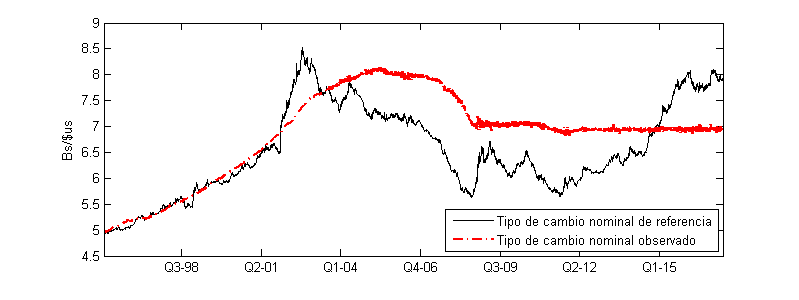
\includegraphics[width=\textwidth]{tcn}
%        \label{tcn}
%\end{figure}

%En efecto, hasta casi finales de 2008 el tipo de cambio nominal fue determinado siguiendo el movimiento de su referencial exceptuando el momento en el que la crisis económica de Argentina generó presiones de depreciación en esta variable.\footnote{Desde la perspectiva de la regla cambiaria siguiendo el tipo de cambio referencial, los tomadores de política interpretan los picos generados por las crisis como pasajeros y deciden no seguirlos, mas bien parecen continuar con la tendencia previa hasta ya pasados los efectos de la crisis. Específicamente, durante la crisis Argentina de 2002 que chocó fuertemente a Bolivia, los tomadores de decisión bolivianos decidieron continuar con una leve depreciación en niveles ya determinados que se prolongó hasta pasada dicha crisis.} Como ha sido ya mencionado, después de mediados de 2003 Bolivia consiguió el equilibrio de su balanza comercial que sería seguido por un ciclo de superávits. Durante este periodo se genera un comportamiento de ``u'' invertida del tipo de cambio nominal que parece indicar que los tomadores de decisión buscaron retomar la regla cambiaria en una situación en la que el tipo de cambio nominal y de referencia se encontraban desalineados. El \emph{catching up} de dicha variable se dio a mediados de 2008. En el cuarto trimestre del mismo año, afrontando la crisis financiera internacional, Bolivia decide mantener su tipo de cambio nominal constante, interpretando el cambio de dirección sugerido por la crisis como transitorio. A pesar que durante 2011 se aprecia levemente la moneda boliviana, la regla cambiaria que buscaba conciliar los tipos de cambio nominal y referencial es abandonada a pesar de que este último sugería la depreciación sostenida, el cual es el comportamiento que la mayoría de las economías de la región presentaron en dicho periodo.

%Este cambio de dirección de la política cambiaria implicó la notable des-dolarización de la economía boliviana, debido a que permitió cambiar las expectativas que la población tenía con respecto al tipo de cambio nominal. Previo a 2005, el régimen de \emph{crawling peg} permitía a la población esperar que el boliviano se devalúe constantemente, en una economía pequeña y altamente dolarizada esto implicaba una perdida constante del poder de conservación de valor de la moneda nacional y sugería al dólar americano como principal instrumento financiero y fiduciario para conservar riqueza e incluso efectuar transacciones monetarias grandes. Desde finales de 2008, los efectos de la significativa apreciación fueron evidentes, estos implicaron que la moneda boliviana podía no solo mantener valor sino también generarlo frente al dólar americano, la principal divisa en el mundo. La posterior estabilidad cambiaria implicó el anclaje de la expectativa del valor del boliviano que junto a otras medidas adyacentes contribuyeron a que sea la principal moneda circulación en Bolivia para el ahorro, crédito y transacciones monetarias. Al no depreciarse constantemente, los precios de bienes importados y derivados de los mismos dejaron de inflarse por efecto de dicho efecto cambiario dando espacio de acción a la política monetaria doméstica. Además, el rendimiento del comercio externo demostró buenos resultados con la inducción de esta política heterodoxa.

%La regla cambiaria utilizada basada en el tipo de cambio de referencia sugiere que Bolivia tiene como objetivo de política cambiaria mantener la competitividad del sector externo y que el tipo de cambio es uno de los instrumentos para lograrlo. Sin perdida de generalidad se puede observar que este ha sido un paradigma importante de política económica en Bolivia siempre buscando generar el valor agregado y captación de divisas a través del fomento de las exportaciones. La bonanza de la economía boliviana de los últimos años ha demostrado que su salud depende de su posición acreedora en la balanza comercial. Estas evidencias delimitan una serie de cuestiones importantes en el tema de efectividad de las políticas económicas llevadas a cabo. ¿Es el tipo de cambio real de equilibrio aquel que determina el balance entre las exportaciones e importaciones?. ¿Cuál es el tipo de cambio real que permite la consecución de este objetivo?. ¿Es el tipo de cambio nominal el instrumento efectivo que permite el movimiento del tipo de cambio real?. 

%Son estas las cuestiones que motivan el análisis de la política cambiaria boliviana y muy en especial la tendencia de equilibrio del tipo de cambio real del país. A continuación, se estima y analiza bajo los métodos de BEER y una variación de FEER (DEER) las medidas de TCR de equilibrio de corto y mediano plazo. No se realiza el análisis de largo plazo porque es considerado poco significativo para la economía boliviana que aún se encuentra en vías de desarrollo y donde aún no se tiene indicios claros del camino de desenvolvimiento pertinente que contribuya a su crecimiento sostenido y sustentable siendo este último la senda de \emph{steady state} en \emph{stricto sensu} que no es aún vislumbrada. Asimismo, se discute ideas centrales de política cambiaria, se plantean posibles desaciertos, miopía conceptual y se introduce la idea de subvaluación estructural de la moneda en una economía determinada por un fuerte contrabando (importaciones ilegales).

Bajo esta motivación el presente documento plantea la consideración de elementos importantes del tipo de cambio real y de la medición de su equilibrio en la sección \ref{pre}; posteriormente, se define la metodología a ser utilizada la sección \ref{tcr}; la verificación de series estadísticas, hechos estilizados y resultados son planteados en la sección \ref{calc}; se continúa con la reflexión de los resultados encontrados en la sección \ref{consid} y para sintetizar lo estudiado, la sección \ref{concl} concluye el documento.



\section{Revisión de Literatura}\label{pre}

\subsection*{Tipo de cambio real}
%TCR
El tipo de cambio real es la variable que refleja cuánto de una canasta básica doméstica es necesaria para comprar una canasta básica extranjera. Esta variable es determinada por la siguiente relación:
\begin{equation}\label{tcr1}
Q_t=E_t\frac{P_t^*}{P_t},
\end{equation}
donde $Q_t$ es el tipo de cambio real, $E_t$ es el tipo de cambio nominal, $P_t^*$ representa el índice de precios de una canasta básica representativa de una economía extranjera y $P_t$ es el índice de precios de una canasta básica doméstica representativa. En logaritmos la expresión \ref{tcr1} es representada por:
\begin{equation}\label{tcrlog}
q_t=e_t+p_t^*-p_t.
\end{equation}
Nótese que las minúsculas describen a la variable en logaritmo. Tanto las expresiones \ref{tcr1} y \ref{tcrlog} representan el poder de compra de una moneda frente a otra. El tipo de cambio real también puede ser analizado en términos de precios transables y no transables.\footnote{En realidad, todas expresiones procuran medir la siguiente relación original de tipo de cambio real medida entre precios no transables y transables $Q_t=\frac{P_{NTt}}{P_{Tt}}$.} Para tal efecto, en el caso de la ecuación \ref{tcrlog} se asume que $p_t=\alpha p_{Nt} + (1-\alpha)p_{Tt}$, donde $0<\alpha<1$, $\alpha=\alpha^*$, en este contexto, $p_{Nt}$ es el precio de no transables, $p_{Tt}$ el de transables y $\alpha$ es la proporción de precios de bienes no transables que constituyen el índice de precios. Entonces:
\begin{equation}\label{tcr2}
q_t=q_{Tt}+\alpha(\hat{p}_{Nt}-\hat{p}_{Tt}),
\end{equation}
donde, el circunflexo implica la diferencia de la variable entre precios domésticos y extranjeros, por ejemplo $\hat{p}_{Nt}=p_{Nt}^*-p_{Nt}$, y $q_{Tt}$ es el tipo de cambio real de bienes transables donde $q_{Tt}=e_t+p_{Tt}^*-p_{Tt}$. Por lo general, se asume que $q_{Tt}=0$ (o $Q_{Tt}=1$) debido a que los precios transables, por el concepto de competitividad y bajo los mismos supuestos de competencia perfecta, tendrían el mismo valor tanto en la economía doméstica como en el exterior dado un tipo de cambio. 

Las ecuaciones \ref{tcr1} y \ref{tcrlog} son análogas e implican que, manteniendo todo lo demás constante, los incrementos de tipo de cambio nominal (devaluación nominal) o de los precios extranjeros o las caídas del nivel de precios local determinan una depreciación real de la moneda nacional. Lo contrario aplica para el caso de una apreciación real. Sin embargo, desde la perspectiva caracterizada en la ecuación \ref{tcr2}, el tipo de cambio real de bienes transables y la diferencia del nivel de precios no transables, y transables, entre el resto del mundo y la economía local determinan los movimientos del TCR. 

La ecuación \ref{tcr2} implica una perspectiva más analítica para estudiar la influencia de las políticas económicas sobre el TCR a través del efecto que generan en los grupos de precios especificados. Por ejemplo, el caso más estudiado entiende que el gasto público (política fiscal) se ejecuta sobre la compra de bienes no transables. Este shock de demanda sobre en el mercado de bienes no transables hace que los precios se incrementen. 

Por otro lado, la teoría contemporánea no describe cual es el efecto de las otras políticas económicas sobre cada conjunto de bienes. Sin embargo, a continuación se ensayan algunas consideraciones al respecto. El impulso de la política monetaria (sin tomar en cuenta los efectos asimétricos sobre el nivel de precios) afecta en mayor medida a los precios no transables, como servicios y bienes locales cuyos precios dependen del dinamismo de la economía nacional y la inflación. En contraposición, los niveles de precios transables son determinados en mayor medida por los mercados internacionales teniendo en cuenta el análisis de comercio externo. Aquí se debe considerar el concepto de homogeneidad de los bienes transables, lo cual implica que todos estos sean iguales y de la misma calidad independientemente de su origen haciendo que sus precios sean los mismos. Sin embargo, en la realidad, se debe considerar que los bienes transables manufacturados tienen diferencias en costos y calidad lo que hace que sus precios difieran sustancialmente incluso estandarizando por moneda el precio de ellos. 

Asimismo, la política cambiaria o el movimiento de las paridades de moneda tienen efecto en los bienes transables debido a que la depreciación (apreciación) cambiaria encarece (abarata) el valor del bien en moneda local. Nótese que en este caso, los países afrontan un amplio nivel de exogeneidad en el sentido que la apreciación de la moneda de un país extranjero, del cual se importan bienes, implicará la depreciación implícita de la moneda local. Finalmente, se debe considerar el efecto que las políticas sociales, comerciales, financieras y laborales tienen afectando la competitividad de los precios finales de los bienes transables a través de la modificación de los costos a los que los productores acceden. 

Es importante destacar que en la teoría económica moderna se entiende que la política económica no tiene influencia en el cambio de tendencia del equilibrio de largo plazo del tipo de cambio real. Esto porque, dados los niveles de los fundamentos, la tendencia y el equilibrio estarían dados. En contraposición, el papel de la política económica está orientada en influir en los fundamentos para que el tipo de cambio real retorne a su nivel de equilibrio cuando se encuentre desequilibrado. Esta perspectiva implica que no se puede estar desviado del nivel de equilibrio por mucho tiempo. Sobre como influir en el movimiento del tipo de cambio real se ampliará la discusión en la sección \ref{consid}.

Entonces, como se ha anotado previamente, las representaciones del tipo de cambio real de las ecuaciones \ref{tcrlog} y \ref{tcr2} son importantes por distintas razones. La primera, que está basada en el propio concepto de la variable, es utilizada para construir estadísticamente el indicador pertinente que caracteriza dicha variable. Por otro lado, la segunda expresión permite realizar una interpretación sobre las fuerzas que podrían influir en sus movimientos.

En este sentido, hay algunas consideraciones prácticas al respecto del tipo de cambio real que deben ser apuntadas. En particular, $p_t^*$ y $p_t$ no siempre representan precios de las mismas canastas básicas, esto porque distintos países consumen distintos bienes básicos, o en otras palabras, no todas las economías incluyen exactamente los mismos productos en sus canastas. Adicionalmente, esto se puede deber a que frente la modernización y aparición de nuevos bienes, los institutos de estadística tardan en actualizar los productos que deberían entrar en la canasta básica. En teoría, esto podría ocasionar algún ruido en el cálculo del tipo de cambio real que en promedio puede asumirse insignificante, aunque queda la duda hasta qué punto esto es perjudicial cuando una convergencia tarda en suceder.\footnote{Por ejemplo, ¿es relevante entre 2010-2017 incluir los servicios de telefonía pública (cabinas fijas y ambulantes), videoreproductor, VHS, minicomponente, walkman, discman y tantos otros dentro de la canasta básica?} Por otro lado, cuando se relaciona al TCR con el comercio internacional de, por ejemplo, materias primas, parece que esta medida cambiaria no tiene incumbencia pues, como ha sido expuesto, mide la relación de bienes que entran dentro de la canasta básica, a la cual las materias primas y demás insumos productivos son ajenos pero altamente comercializados internacionalmente. Finalmente, a pesar que algunos investigadores asumen que $q_{Tt}=0$, debido al supuesto de perfecta sustitubilidad de bienes transables por la noción de competencia perfecta de transables, en este documento se considera importante tomar en cuenta la diferenciabilidad horizontal y vertical de bienes transables por lo menos al momento de realizar consideraciones derivadas de los resultados.

\subsection*{Tipo de cambio real de equilibrio}

Dada la definición del tipo de cambio real es preciso establecer la definición de su correspondiente equilibrio. El mismo es una variable no observada que idealmente podría ser considerada como el contrafactual positivo\footnote{Desde la perspectiva deontológica de la ciencia.} del tipo de cambio real. En otras palabras, es la variable que captura los valores ideales o en equilibrio de los componentes que conforman el TCR. En este sentido, se entiende como valor de equilibrio al tipo de cambio real que representa a la economía abierta que está en equilibrio tanto a nivel interno como externo. Las implicaciones de estar en equilibrio son discutibles porque implica distintas interpretaciones dependiendo de la perspectiva del autor.

El propio hecho que una variable denominada tipo de cambio real de equilibrio exista, indica que la ciencia social acepta tanto teórica como empíricamente que el tipo de cambio observado no corresponde a los valores de equilibrio de los mercados que lo definen. En este sentido, se entiende que existen distorsiones (transitorias o inesperadas) en dichos mercados que generan valores observados que podrían no corresponder a lo que deberían representar y en el peor de los casos retroalimentarse debido a algún tipo de persistencia. El hecho de reconocer esto implica asumir una postura teórica para identificar las distorsiones transitorias o no anticipadas. A su vez esto determinará el tipo de equilibrio que se considere y el consecuente método para calcularlo.

%Eq CP MP LP
Bajo esta premisa, \cite{driver2005concepts} distingue tres tipos de conceptos centrales de equilibrio utilizados y operativizados por distintos autores. Los de corto plazo que capturan movimientos de la serie correspondientes a los de sus fundamentos y a factores transitorios abstrayendo únicamente los shocks inesperados. Los de mediano plazo que se caracterizan por su compatibilidad con el balance externo e interno de la economía, es decir, esta perspectiva es consistente con los fundamentos en su nivel tendencial, los mismos que pueden estar aún convergiendo, o no, a sus valores de estabilidad de largo plazo. Y, finalmente, el equilibrio de largo plazo que ocurre en pleno empleo y es compatible con los co-movimientos de los valores de largo plazo de sus fundamentos, en otras palabras, cuando no hay cambio endógeno de tendencia.

El concepto de equilibrio de corto plazo implica que los mercados están en equilibrio pero son afectados por impulsos transitorios y shocks inesperados. La remoción de estos últimos elementos constituye el objetivo operativo de estos modelos para encontrar el equilibrio. El concepto de mediano plazo, asume que los datos observados podrían no corresponder al equilibrio en los mercados que los generan; para contrastar esta hipótesis se encuentra la diferencia entre los niveles asumidos de equilibrio del sector interno y externo y los compara con los niveles tendenciales de las variables observadas. Finalmente, el concepto de largo plazo implica que para obtener el nivel de equilibrio del TCR todos los mercados y las correspondientes variables deberían estar en pleno empleo, entonces, a partir de los datos observados se construye una estructura de la economía que aproxima las interelaciones de las variables capaces de reproducir la conducta de la economía para entonces generar los valores de equilibrio abstrayendo los shocks inherentes de las series observadas.

%Eq interno externo
Entonces, asumir que el mercado interno y externo están siempre en equilibrio, y los datos observados son una reproducción de dicha relación, implica asumir un supuesto importante para determinar el concepto de equilibrio que vaya a ser ejercitado. En tal sentido, se propone utilizar ambas nociones, una que asuma que los mercados efectivamente están siempre en equilibrio y otra que asuma la existencia de un equilibrio más allá de lo observado. Sin embargo, antes de discutir estas perspectivas a profundidad se plantea revisar algunos matices de las características de los conceptos.

Con respecto a la perspectiva de largo plazo en la que los valores que se deben utilizar para encontrar la senda de equilibrio son los de \emph{steady-state} y pleno empleo, se debe establecer las siguientes consideraciones. Dichos resultados idealizados son obtenidos con base en valores pasados de las variables de la economía que determianrían el crecimiento vegetativo de una economía en particular. Esto implica pensar que la población crecerá a una tasa constante al igual que los niveles de capital y trabajo mientras que básicamente todas las decisiones económicas en el sistema convergerán a reproducirse constantemente a través de la repetición sin cambios en las mismas. 

Esto implica conocer la estructura del proceso generador de datos de la economía en particular. Se debe convenir que una economía y sus realizaciones no son simplemente el hecho de interacciones simplificadas de sus agentes, sino que cambios y diferentes direcciones son determinadas en la complejidad y heterogeneidad de los sistemas que la componen. Asimismo, se debe reconocer que los ámbitos políticos, culturales y sociales también tienen una influencia importante en el área económica. Todo esto sin tomar en cuenta los shocks exógenos e inesperados que puedan suceder.

En tal sentido, el trabajo de identificación de los sistemas macroeconómicos ha avanzado bastante en el contexto de países desarrollados. En estos últimos las relaciones económicas productivas ya están  consolidadas en sus mercados internos y en los mercados internacionales habiéndoles concedido la sostenibilidad de su desarrollo, lo cual facilita y hace más creíble el supuesto de convergencia a largo plazo. Esto debido su mejor alternativa es continuar replicando la fórmula explotando el aspecto de su economía en el que son más competitivos que el resto de los países y con el que les va bien internamente. 

En países en desarrollo, el alcance de estos métodos estadístico es limitado para estos fines por el estudio poco particular de dichas economía. Se debe recordar que existen características persistentes que hacen que sus niveles de desarrollo se ubiquen por detrás de otras economías haciendo que los procesos productivos y relaciones económicas sean muchas veces precarias, de corto plazo y oportunistas. Entonces, la revisión estadística de los datos de estos países generaría resultados subóptimos situándolos siempre en la misma condición de desarrollo insuficiente a pesar de estar aplicando políticas para revertir esta situación para mejorar su posición internacional buscando el mayor bienestar posible de sus habitantes. 

Para caracterizar este punto, suponga la situación en la que se utiliza la identificación de una economía avanzada y se pretende que es una aproximación que también corresponde a la de una economía en desarrollo con características bastante particulares. Esto sería como estimar la distancia de los trancos de un caballo con base en un modelo que replica los pasos de un humano. Por lo tanto, se procura la estimación del TCR de equilibrio en modelos más adecuados y que sean capaces de capturar las particularidades de la economía analizada.


\subsection*{Importancia del equilibrio}
%Por qué es necesario medir el equilibrio
La literatura especializada en la determinación de un tipo de cambio real de equilibrio es vasta y reúne una variada cantidad de definiciones, métodos y consideraciones especiales al respecto. Por ejemplo, \cite{driver2005concepts} propone que el fin de estas prácticas en economías con tipos de cambio poco flexibles es determinar el costo de mantener esta variable relativamente fija. Adicionalmente, realizar el cálculo permitiría entender cuales son los principales \emph{shocks} externos que mueven la trayectoria de la variable fuera de su equilibrio y cuales son las variables que influyen en su movimiento \citep{macdonald2000concepts}. Esta perspectiva está basada en el supuesto de que economías con tipo de cambio flexible estarían siempre alrededor de su valor real de equilibrio por estar definidas libremente en sus mercados mediante el equilibrio de los mismos. Por otro lado, la importancia conceptual de representar el equilibrio tanto interno como externo permitiría verificar la fortaleza de la moneda tanto local como internacionalmente \citep{akrama2003real}.

En este caso particular, con base en las consideraciones históricas, se plantea estimar el tipo de cambio real de equilibrio que internalice el fin último de política económica en Bolivia que es la obtención de superávits de balance comercial y cuenta corriente. Al mismo tiempo, se pretende estimar cuales son las fuerzas económicas que mueven el valor de tipo de cambio real.

\subsection*{Metodologías}
%Basado en los surveys corto conciso y finalmente analítico concentrarse no en describirlos pero en los pros y contras
Como ha sido adelantado, hay una variedad de métodos de los cuales se puede escoger dependiendo de la finalidad y alcance que se quiere dar a la perspectiva de estudio. \cite{driver2005concepts}, \cite{macdonald2000concepts} y \cite{akrama2003real} ofrecen una buena recolección de métodos. Los equilibrios obtenidos las metodologías son distintos entre ellos. La razón se basa en el hecho que cada una está determinada por diferentes supuestos y conceptos de equilibrio. Ya cerrada la discusión acerca del uso de \emph{steady-state} y pleno empleo se concluye que para los fines analíticos del presente documento, se enfocará el estudio a los modelos de corto y mediano plazo. Por lo tanto, se procederá a revisarlas y escoger a las que se constituyan ser las más apropiadas desde la perspectiva económica de Bolivia.

En el corto plazo se distingue particularmente los métodos PPC y \emph{behavioral equilibrium exchange rate} BEER. El primero está basado en el cumplimiento de la condición de poder de paridad de compra. Sin embargo, esta alternativa no es realista debido a que no existe la completa flexibilidad de precios que permita que la condición se cumpla a cabalidad existiendo bloqueos y distorsiones estructurales a través de impuestos y aranceles, por otro lado, también se puede citar la diferenciación horizonal y vertical de los bienes transables como una razón por la que esta condición no se cumpla. Adicionalmente, el efecto \emph{Balassa-Samuelson} propone que el efecto de los precios descompuestos entre transables y no-transables \citep{balassa1968effective} es importante en la definición del tipo de cambio real, mientras que a través de esta perspectiva no se observa dicha caracterización. Trabajos empíricos indican que de cumplirse, esta relación lo haría en el largo plazo. Confirmando el rechazo de esta hipótesis, investigaciones empíricas en Bolivia como \cite{lora2000tipo} y \cite{humerez2005reexaminando} descartan su aplicación.

La siguiente alternativa es el modelo BEER que se basa en determinar el equilibrio de tipo de cambio comportacional determinado por sus fundamentos. Este modelo es asociado con el trabajo de \cite{clark1999exchange}. La idea es establecer la relación de cointregración entre el tipo de cambio real y sus fundamentos, dado que estas variables al ser integradas en primer grado podrían compartir la tendencia en una relación de largo plazo que es implementada por un modelo de corrección de errores que mide de los efectos de corto plazo en la inter-relación de las variables. Asimismo, este modelo permite determinar como es que los fundamentos explican los movimientos de corto plazo en la relación de equilibrio.

Esta será la perspectiva de corto plazo que se utilizará para hallar el tipo de cambio real de equilibrio. La identificación original de \cite{clark1999exchange} se basa en el cumplimiento de la paridad encubierta de tasas de interés, sin embargo, hay otros tipos de identificación que desembocan a estimaciones similares.

Con respecto al equilibrio de mediano plazo, se analizan las principales opciones determinadas por la literatura. En esta línea existen dos corrientes de estimación con sus respectivas variantes. En primer lugar, los modelos de equilibrio permanente, y en segundo lugar, los de equilibrio de fundamentos. Estos últimos implican un balance tanto interno como externo con el cual determinan una trayectoria de tendencia normativa de la economía. Típicamente son conocidos como \emph{fundamental equilibrium exchange rate} FEER. En segundo lugar, están los modelos \emph{permanent equilibrium exchange rate} PEER, que extiende el modelo BEER, y \emph{atheorical permanent equilibrium exchange rate} APEER. Según \cite{driver2005concepts}, ambos son métodos que están basados en conceptos de mediano-largo plazo y son más estadísticos que económicos, por esta razón se decide enfocarse simplemente en los de la familia FEER.

El equilibrio en los modelos FEER ocurre cuando cierto nivel de tipo de cambio real permite el logro de los niveles de cuenta corriente norma y PIB en sus niveles de tendencia, de esta manera, se consigue el equilibrio interno y externo. Existe una variedad de métodos de estimaciones FEER, las mismas se diferencian en sus maneras de establecer la mejor forma de conciliar el equilibrio externo con el interno haciendo uso de las distintas ``normas'' de cuenta corriente y ``valores subyacentes'', entre estos se puede distinguir el balance macroeconómico y la sostenibilidad externa \citep{bussiere2010methodological}. Sin embargo, se ha distinguido el carácter normativo de la política fiscal en el modelo a través de las variables ``normas'' y ``valores subyacentes''. Esta última consideración ha generado que se establezca el modelo \emph{desired equilibrium exchange rate} DEER como variación de FEER, siendo que este último plantea el uso de una política económica óptima para la consecución del objetivo de político definido en el modelo.

El sentido de normatividad en componentes de norma y subyacente para FEER implica asumir supuestos y adoptar como meta de equilibrio económico las condiciones que el balance macroeconómico y la sostenibilidad externa proponen bajo el marco estadístico de los datos observados. Por esta razón y porque se conocen los objetivos de la política económica boliviana se encuentra conveniente utilizar DEER. Hay dos metas que los hacedores de políticas bolivianos han tenido desde 1985, estas son limitar la variabilidad del producto permitiendo una tendencia de crecimiento positiva y sostenida y que la balanza comercial presente equilibrio o en el mejor de los casos superávit caracterizando de este modo una cuenta corriente positiva.

Entonces, dado el repaso de las metodologías existentes y tomando en cuenta la pertinencia de ellas para su aplicación en el caso boliviano, se aplicará la metodología BEER y DEER para realizar la estimación del tipo de cambio real de equilibrio. 

%\subsection*{Evidencia empírica internacional}
%La mayoría de esta literatura no solamente es el paper teórico sino tambien la aplicación
%Países desarrollados
%Países emergentes
%Países en desarrollo
%Países de la región


\subsection*{Evidencia empírica en Bolivia}
%Qué se ha hecho
Acompañando la búsqueda del cometido que se tiene en el presente documento se ha revisado la evidencia de investigaciones en Bolivia en la búsqueda de la determinación del tipo de cambio real de equilibrio. En tal sentido se hace referencia a \cite{ferrufino1992tipo}, \cite{marquez2003estimacion}, \cite{humerez2005reexaminando}, \cite{montiel2007equilibrium}, \cite{cerutti2008bolivia}, \cite{mendieta2008equilibrio}, \cite{bello2010tipo}, \cite{cerezo2010desempeno} y \cite{cerezo2011tipo}. Existen grandes similitudes entre todas las investigaciones generadas especialmente después de 2000. En primera instancia, el objetivo central de ellos es estimar los desalineamientos con respecto al equilibrio, y en segundo lugar, todos presentan una metodología similar.

%Metodología + resultados importantes
Los documentos que presentan estructura de identificación son aquellos previos al 2005. Específicamente, se hace referencia a \cite{lora2000tipo}, citada también por \cite{marquez2003estimacion} la misma que se constituye en la principal sistematización teórica que justifica el comportamiento del tipo de cambio real. Esta identificación está basada en el trabajo analítico de \cite{baffes1999red} y \cite{hinkle1999exchange} que asocia la demanda de trabajo en los sectores transables y no transables de una economía y la producción generada por los mismos junto con los componentes de la cuenta corriente y el comportamiento del gobierno. Adicionalmente, \cite{humerez2005reexaminando} utiliza la identificación de \cite{elbadawi1994estimating} a partir de las identidades y relaciones de cuentas nacionales. La aplicación empírica de estos modelos se realiza a través de modelos de cointegración.

Los documentos posteriores no presentan claramente una estrategia de identificación, sin embargo, heredan el método empírico de medición original a través de la cointegración y se concentran en probar la inclusión de distintos fundamentos en la relación de estudio y ampliar la base de datos, siendo que esta última no está unificada entre las investigaciones analizadas. Por este motivo, es que se puede concluir que para estos trabajos la identificación del movimiento del TCR determinado por sus fundamentos es no estructural. Al mismo tiempo, se podría proponer que siguen una visión de estimación reducida, que es como puede ser identificada estas metodologías en la literatura pertinente. Sin embargo, se debe destacar que a pesar de que no se propone una estructura particular para el caso boliviano, estos modelos de cointegración son similares a los generados a través de los modelos BEER.

Entre estos trabajos se debe destacar a \cite{cerezo2011tipo} que además del acostumbrado modelo de cointegración de fundamentos adiciona otras perspectivas analíticas más que le permiten estimar distintas trayectorias de equilibrio del TCR a través de: el método de equilibrio macroeconómico, sostenibilidad externa, un modelo que procura calcular el efecto Penn-Balassa Samuelson y un modelo de equilibrio general.

Los primeros dos métodos adicionales del documento citado de \cite{cerezo2011tipo} son distintas perpectivas de FEER como puede constatarse en \cite{bussiere2010methodological}.\footnote{A pesar de que \cite{bussiere2010methodological} exponen los métodos para calcular la cuenta corriente norma que pertenecen a la familia de métodos FEER, la principal fuente metodológica de \cite{cerezo2011tipo} es \cite{isard2007equilibrium}} Estos modelos ofrecen una medición para el periodo 2010 por la naturaleza parcial que los mismos modelos tienen, lo cual es algo recurrente cuando se lleva a cabo este método. Bajo esta metodología obtienen una subvaluación de 1\% y 0,8\% para los métodos denominado equilibrio macroeconómico y sostenibilidad externa, respectivamente. De la misma manera, el modelo que estima el efecto Penn-Balassa Samuelson (que procura encontrar el efecto Penn a través de un modelo de sección cruzada) es ejecutado para calcular una subvaluación de 16\% para el año 2010. Mientras que con los restantes dos métodos (BEER y DSGE) consiguen determinar una serie para el TCR de equilibrio durante el periodo para el que tienen datos. A propósito del modelo DSGE, se aduce una identificación basada en el modelo escandinavo de inflación, los modelos intertemporales de los 80's y la literatura de los ciclos reales.

%\begin{landscape}
\begin{table}
\begin{center}
\caption{Lista de Fundamentos de TCR en Bolivia}\label{otros}
\resizebox{\textwidth}{!}{%
\begin{tabular}{lccccccccc}									
\hline
\hline													
Estudio	&	 Lora	&	 Aguilar	&	 Humerez	&	 Montiel	&	 Mendieta	&	 Cerutti	&	 Bello	&	 Cerezo	&	 Cerezo	\\

	&	 2000	&	 2003	&	 2005	&	 2007	&	 2008	&	 2008	&	 2010	&	 2010	&	 2011	\\
	
\hline										
Años de estudio	&	 1988-1999	&	 1990-2002	&	 1990-2003	&	 1969-2005	&	 1991-2007	&	 1990-2006	&	 1969-2006	&	 1992-2009	&	 1990-2010	\\

Periodicidad	&	 Trimestral	&	 Trimestral	&	 Trimestral	&	 Anual	&	 Trimestral	&	 Trimestral	&	 Anual	&	 Trimestral	&	 Trimestral	\\

\hline
 Gasto público	&	-	&	-	&		&		&	+	&	+	&		&	+	&	+	\\
\hline
 Términos de intercambio	&	-	&	-	&	-	&	-	&	-	&	-	&	-	&	-	&	-	\\
\hline
 Política Comercial	&	-	&	+	&		&		&	-	&		&		&		&		\\
\hline
 Balanza Comercial	&		&		&		&		&	-	&		&		&	+	&	-	\\
\hline
 Flujos de Capital	&	-	&	-	&	+	&		&		&	-	&		&		&		\\
\hline
 Apertura Comercial	&	+	&	+	&	+	&		&		&		&	+	&		&		\\
\hline
 Diferencial de tasas de interés	&		&	-	&		&		&		&		&		&		&		\\
\hline
 Productividad	&		&		&		&	-	&	+	&	-	&		&		&		\\
\hline
 Libor	&		&		&	+	&		&		&		&		&		&		\\
\hline
 Dummy (94-95)	&	+	&	+	&		&		&		&		&		&		&		\\
\hline
 IPC externo	&	+	&		&		&		&		&		&		&		&		\\
\hline
 Precio del Gas	&		&		&		&		&		&		&		&		&	-	\\
\hline
 RIN	&		&		&		&		&		&		&		&		&	-	\\
\hline
 NFA	&		&		&		&		&		&	-	&		&		&		\\
\hline
Sobrevaluado	&	 98-99	&	 90-93, 97-99	&	 91-93, 98-00, 02	&	 81-00	&	 91-93, 99-04	&		&	 81-85, 98-05	&	 97-03, 08-09	&	 94-01, 02	\\
Subvaluado	&	 94-96	&	 94-95, 00-01	&	 93-95, 01	&	 70s, 2000s	&	 94-95, 05-06	&		&	 86-97	&	 93-96, 03-08	&	 07-10	\\
Sobrevaluado	&		&		&		&		&		&		&		&		&	 08-09	\\
Subvaluado	&		&		&		&		&		&		&		&		&	 05-06, 09-10	\\
\hline
\hline
\end{tabular}%
}
\end{center}
\begin{scriptsize}
\emph{Nota:} Elaboración propia con base a los documentos previamente citados.
\end{scriptsize}					
\end{table}	
%\end{landscape}

El conjunto de documentos revisados, al tener metodologías de cálculo similares pueden ser comparados a través de la inclusión de variables explicativas como se reproduce en el cuadro \ref{otros}. En este sentido, se encuentra que los términos de intercambio y el gasto público son las variables más robustas a través de las investigaciones, además de ser las que aparecen en la mayoría de las mismas. Después le sigue apertura comercial. La variable que es el componente central para calcular el modelo de BEER clásico que es la diferencia de tasas de interés solo es incluido por una investigación. Asimismo, las investigaciones extranjeras acerca del tipo de cambio real de equilibrio en Bolivia son las únicas que incluyen productividad para aproximar el efecto Balassa-Samuelson, mientras que otra investigación local plantea incluir el PIB per cápita boliviano como proxy de la misma.

Adicionalmente, también se exponen los periodos en los que los modelos de comportamiento encontraron desequilibrios importantes. Varios de estos estudios coinciden que en 1994-1995 hubo subvaluación y en 1998-1999 sobrevaluación. 

%Relevancia de lo ya hecho, si cumple los objetivos
Por otro lado, dada la heterogeneidad en el uso del concepto parece necesario hacer hincapié en lo que el efecto Balassa-Samuelson es y a lo que se refiere. De la ecuación \ref{tcr2} se entiende que $\hat{p}_{Nt}-\hat{p}_{Tt}=\hat{a}_{Tt}-\hat{a}_{Nt}$ donde los $a_t$ se refiere a la productividad económica. esta relación implica que mientras mayor productividad en el sector transable se tenga, mayores presiones a la depreciación habrán, es decir los precios transables de la economía se abaratan. El efecto de la diferencia entre productividades sobre el tipo de cambio real es conocido como el efecto Balassa-Samuelson. Es importante recalcar que para el análisis empírico de la influencia de esta variable en el tipo de cambio real y el cálculo de su equilibrio la disponibilidad de datos distinguiendo la productividad en los sectores transables y no transables por separado es limitada. 

%Analizar lo que falta

\section{Métodos Empíricos}\label{tcr}

La descripción de los métodos  que es realizada a continuación no pretende desglosar la identificación paso a paso. El objetivo es citar los métodos a ser utilizados para la estimación en la parte \ref{calc} del documento, mientras se hacen notar las características más importantes y relevantes de los mismos. En primera instancia se repasa la identificación clásica de BEER, la misma que refleja la necesidad de dar mayor estructura en la inclusión de los fundamentos. En este cometido se debe notar que la crítica a los modelos de PPC reaparece siendo que la paridad de tasas de interés encubierta, en la que la identificación básica de BEER está basada, al igual que la condición de poder de paridad de compra puede que no se de. A priori, se entiende que la parcial movilidad de capitales  en Bolivia es la evidencia necesaria para considerar que la paridad de tasas de interés encubierta no se da en Bolivia. Sin embargo, el propósito de citar la identificación original de BEER es entender el canal por el cual entran los fundamentos,\footnote{El canal, descrito por \cite{clark1999exchange}, es a través de las expectativas de tipo de cambio como se verá más adelante} aunque sea sin estructura. Ya en la identificación del modelo de equilibrio parcial citado, a continuación del original, se aplica la estructura necesaria de una economía modelo abierta y pequeña para justificar la inclusión de los fundamentos. En este punto se debe notar que no se espera que la economía modelo abierta y pequeña sea igual a la de Bolivia, pero en términos generales ambas incluirían en el mejor de los casos las mismas variables, con la diferencia de la estructura en los parámetros duros y, por ende, con direcciones y magnitudes en los parámetros estimados distintos.

La identificación de los modelos FEER y DEER es similar entre ellos. La diferencia está en la normatividad inherente en la versión de objetivos de cuenta corriente de FEER, mientras que DEER permite optimatizar la política económica para obtener los resultados pretendidos. Debido a que Bolivia ha estado procurando la competitividad externa para lograr superávits en cuenta corriente, se utilizará tal objetivo. La identificación DEER será elaborada para mostrar en que casos se utiliza los objetivos deseados de política. Mayores detalles pueden ser encotrados en \cite{james2012handbook}.		

\subsection*{Identificación de BEER}

La identificación clásica del modelo BEER nace de la condición de paridad de tasas de interés encubierta:
\begin{equation}
\mathbb{E}_t[\Delta e_{t+k}]=-(i_t-i_t^*)+\pi_t.
\end{equation}
Utilizar simplemente esta condición impone el reto de incluir en el modelo las expectativas de tipo de cambio, \cite{clark1999exchange} las sustituyeron por las tendencias de los fundamentos.
\begin{equation}
\hat{q}_t=\mathbb{E}_t[q_{t+k}]+(r_t-r_t^*)+\pi_t.
\end{equation}

%Entonces, se define la condición de paridad de tasas de interés encubierta, las minúsculas indican variables en logaritmos:
%\begin{equation}
%\mathbb{E}_t[\Delta e_{t+k}]=-(i_t-i_t^*)+\pi_t,
%\end{equation}
%donde $i_t$ es la tasa de interés nominal doméstica, $i_t^*$ es la tasa de interés nominal extranjera y $\pi_t=\lambda_t+k$ es la premio de riesgo. Esta condición iguala las expectativas de tipo de cambio con el riesgo  \emph{ex ante} ajustado por las tasas de retorno de bienes capitales domésticos y extranjeros. Sumando y restando el diferencial de expectativa de inflación se obtiene:
%\begin{equation}
%\hat{q}_t=\mathbb{E}_t[q_{t+k}]+(r_t-r_t^*)+\pi_t,
%\end{equation}
%donde $r_t=i_t-\mathbb{E}_t(\Delta p_{t+k})$ es el tipo de cambio \emph{ex ante} ajustado por la expectativa de inflación. Asimismo, considérese que la prima de riesgo es dependiente del tiempo y aproximada por:
%\begin{equation}
%\lambda_t=g(\frac{gd_t}{gd_t^*}),
%\end{equation}
%donde $gd_t$ es la deuda pública, como siempre el asterisco indicará que la variable pertenece al extranjero siempre y cuando no se indique otra cosa. Asimismo, la expectativa de tipo de cambio está definida por:
%\begin{equation}
%\hat{q}_t=\mathbb{E}_t[q_{t+k}]=\mathbb{E}_t[\beta' Z_t]=\beta' Z_t,
%\end{equation}
%donde $Z_t$ es el conjunto de fundamentos típicamente entendidos como términos de intercambio, ratio de precios no transables respecto a transables y activos extranjeros netos.

El resultado de dicha identificación genera la siguiente relación:
\begin{equation}\label{qb}
q_t=f(Z_t)+(r_t-r_t^*)+\lambda_t+k,
\end{equation}
en la que no existe ningún supuesto de estructura bajo el cual la inclusión de los fundamentos variables $Z_t$ son admitidos en la relación $f(\cdot)$, lo cual permite experimentar incluyendo y excluyendo fundamentos que se consideren pertinentes. Adicionalmente, $\lambda_t=g(\frac{gd_t}{gd_t^*})$ representa la relación de deuda pública entre la economía local y el extranjero y $k$ es el premio de riesgo. 

De acuerdo a esta identificación, se adelanta que la tendencia de tipo de cambio es su equilibrio y estará definida en mayor o menor medida por los datos históricos que se tenga de esta variable y sus fundamentos, eso quiere decir que siempre se verá que el tipo de cambio está alrededor de su valor de equilibrio y las demás variables incluidas en el modelo determinarán la forma en la que la serie del TCR podrá ser influenciado en la dirección de su equilibrio. Por tanto, desde esta perspectiva, la política económica estará definida en el uso de los fundamentos para cerrar las brechas con respecto al tipo de cambio real de equilibrio. Lo que queda sin identificar es qué fundamentos incluir.

Con al finalidad de responder a esta última cuestión, se opta por modelar el valor del tipo de cambio real de equilibrio a partir de un modelo semi-estructural de equilibrio parcial para una pequeña economía abierta, este planteamiento permitirá delimitar las variables a ser denominadas como fundamentos económicos del TCR. Asimismo, nótese que el modelo propuesto es compatible con el caso boliviano desde una perspectiva macroeconómica y la simplicidad del mismo es necesaria para lograr el cometido citado previamente.

En esencia, se considera como base el modelo de \cite{Calderon2004exchange} que a su vez se enmarca en el modelo de bienes transables y no transables de \cite{Obstfeld1995dynamics}. A continuación, se hará referencia a una pequeña economía abierta que interactúa con un país foráneo. Ambas economías cuentan con un sector de bienes transable y uno no transable. El sector de bienes transables, por simplicidad tiene un sólo bien homogéneo, cuyo precio es definido en los mercados internacionales de forma competitiva. En contraparte, el sector no transable mantiene una estructura monopólica con precios rígidos. Precisamente a partir de este supuesto, la especificación permitirá incorporar como fundamento la productividad entre bienes transables y no transables. 

Un segundo aspecto relevante hace referencia a los representantes de la economía doméstica que estarán dotados de una cantidad constante del bien transable en cada periodo, además tienen el poder monopólico sobre uno de los bienes no transables. Mientras que los productores residen en ambos paises en intervalos definidos. 

Con relación a las preferencias sobre el consumo real y el esfuerzo laboral se definen como idénticas para todos los agentes en el mundo, la simetría en preferencias y restricciones presupuestarias darán lugar a la resolución del problema de optimización del consumidor y productor representativo de la economía doméstica. El modelo considera también la introducción del gobierno bajo el supuesto de que éste sólo consume bienes no transables.  

Según la descripción realizada en \cite{Calderon2002panel} y \cite{Calderon2004exchange}, el agente representativo además puede invertir en instrumentos financieros transables internacionales, específicamente en bonos, por lo que estará sujeto a una restricción presupuestaria que será una función del consumo agregado, la dotación de bienes transables, los precios de los bienes transables y no transables y la tasa de retorno real del instrumento financiero. Hacia adelante, este supuesto permitirá incorporar los activos externos netos como fundamento. Como explica Calderon(2002), las soluciones log-linealizadas del modelo incorporadas a la ecuación del tipo de cambio real permiten definir la siguiente estructura: 

\begin{equation}
\ln q_t=\phi_0+\phi_1\left(\frac{F}{Y}\right)_t+\phi_2\ln\left(\frac{Y_T}{A_N} / \frac{Y_T^*}{A_N^*}\right)_t+\phi_3\ln\left(\frac{P_T^X}{P_T^M}\right)_t+\phi_4\ln\left(\frac{G}{G^*}\right)_t+\mu_t
\end{equation}

En este marco, los fundamentos que explican el tipo de cambio real de equilibrio, serán por un lado el coeficiente de la posición de activos externos netos, la productividad laboral, los términos de intercambio y el gasto de gobierno.  

\subsection*{Identificación de DEER}

El equilibrio en balance externo está basado en la idea que la variación de cuenta corriente está únicamente determinada por la balanza comercial, en este punto se hace abstracción de cualquier otro componente dentro de la Balanza de Pagos que sea influenciada por el tipo de cambio. A su vez, es el tipo de cambio real junto las variables de demanda que determinan los niveles de importaciones y exportaciones, definiéndose las ecuaciones de comercio como:
\begin{equation}\label{X}
X=f(\overset{+}{Y^*},\overset{+}{Q}),
\end{equation}
\begin{equation}\label{M}
M=g(\overset{+}{Y},\overset{-}{Q}).
\end{equation}
Donde $Y^*$ representa al PIB externo, $Y$ es el PIB doméstico, es decir las demandas de exportaciones e importaciones respectivamente,$Q$ es el tipo de cambio real, $X$ son las exportaciones nominales y $M$ las importaciones nominales.
La diferencia de ambas junto con otros ingresos componen la cuenta corriente definida como es usual:
\begin{equation}\label{CC}
CC\equiv(X-M)+Ing1+Ing2
\end{equation}
Donde $Ing1$ e $Ing2$ son las transferencias y rentas respectivamente.
Considérese, entonces, como ya ha sido propuesto que la variación de cuenta corriente únicamente está determinada por cuanto cambie la balanza comercial:
\begin{equation}\label{sup}
\frac{\partial CC}{\partial Q}=\frac{\partial BC}{\partial Q}
\end{equation}
La variación de cuenta corriente es la distancia entre el valor observado y el valor en que idealmente debería presentarse por la barra encima de la variable. A continuación se procede a dividir el lado izquierdo de la condición \ref{sup} por el valor nominal de las importaciones:
\begin{equation}\label{dcc}
\frac{\partial CC}{Q}=CC-\bar{CC}
\end{equation}
La variación de la balanza comercial representada por el lado derecho de la igualdad de \ref{sup} puede ser expresada como la variación de volúmenes reales. Donde la balanza comercial es:
\begin{equation}
BC=\frac{P_X X}{PIB}-\frac{P_M M}{PIB}.
\end{equation}
Derivándola respecto al tipo de cambio real:
\begin{equation}
\frac{\partial BC}{\partial Q}=\frac{\partial X}{\partial Q} \frac{P_X}{PIB}+\frac{\partial P_X}{\partial Q} \frac{X}{PIB} - \frac{\partial M}{\partial Q} \frac{P_M}{PIB}-\frac{\partial P_M}{\partial Q}\frac{M}{PIB},
\end{equation}
donde $\frac{\partial P_X}{\partial Q}=0$ debido a que los precios de las exportaciones están en moneda doméstica y $\frac{\partial P_M}{\partial Q}=-\frac{P_M}{Q}$ implica elasticidad unitaria respecto a $Q$.

Entonces, se obtiene que:
\begin{equation}\label{partialq}
\frac{\partial BC}{\partial Q}=\frac{1}{Q} \left[\eta_X \frac{P_X X}{PIB}-(\eta_M -1)\frac{P_M M}{PIB}\right].
\end{equation}

Sustituyendo \ref{dcc} y \ref{partialq} en \ref{sup} y despejando $Q$ se obtiene la variación del tipo de cambio real necesaria para tener la cuenta corriente deseada $\bar{CC}$.

%A continuación se transforma a logaritmos:
%\begin{equation}
%\mathrm{d}BC=P_XX\frac{\mathrm{d}X}{X}-P_MM\frac{\mathrm{d}M}{M}
%\end{equation}
%Lo cual es expresado como:
%\begin{equation}
%\mathrm{d}BC=P_XX(\varepsilon_xq+\eta_xy^*)-P_MM(\varepsilon_mq+\eta_my)
%\end{equation}
%Utilizando la misma estrategia que en \ref{dcc}:
%\begin{equation}
%\frac{\mathrm{d}BC}{P_MM}=\frac{P_XX}{P_MM}(\varepsilon_xq+\eta_xy^*)-\frac{P_MM}{P_MM}(\varepsilon_mq+\eta_my)
%\end{equation}
%Reemplazando el ratio exportaciones - importaciones por la variable $\tau$ y simplificando:
%\begin{equation}\label{dbc}
%\frac{\mathrm{d}BC}{P_MM}=\tau(\varepsilon_xq+\eta_xy^*)-\varepsilon_mq-\eta_my
%\end{equation}
%Cuando se igualan las ecuaciones \ref{dcc} y \ref{dbc}, y se resuelve para $q$ se encuentra que:
%\begin{equation}\label{r}
%q=\frac{1}{\mu(\tau\varepsilon_x-\varepsilon_m)}[cc-\mu(\tau\eta_xy^*-\eta_my)-cc^*]
%\end{equation}
%Las ecuaciones de comercio son definidas por:
%\begin{equation}
%X=Y^{*\eta_x}Q^{\varepsilon_x}
%\end{equation}
%\begin{equation}
%M=Y^{\eta_m}Q^{\varepsilon_m}
%\end{equation}
%\begin{equation}
%\mathrm{d}x=\eta_x\mathrm{d}y^*+\varepsilon_x\mathrm{d}q
%\end{equation}
%\begin{equation}
%\mathrm{d}m=\eta_m\mathrm{d}y+\varepsilon_m\mathrm{d}q
%\end{equation}

En este caso se debe reiterar que los modelos típicos FEER generalmente utilizan valores norma y subyacentes para estimar el cierre de brecha de la cuenta corriente generado por el tipo de cambio real de equilibrio. En esta perspectiva metodológica particular denominada genéricamente DEER se utiliza la cuenta corriente observada y como objetivo una cuenta corriente que reemplaza los déficits observados por niveles de balance nulo y admite niveles de superávit suavizándolos. Esto implica que este modelo pretende estimar un tipo de cambio real de equilibrio que no admite déficits y que permite superávits sin variabilidad. 


%Función de utilidad 
%\begin{equation}
%U_t=\sum_{t=0}^\infty \beta^t \left( \frac{\sigma}{\sigma - 1} %C_t^{\frac{\sigma-1}{\sigma}} - \frac{k}{2} l_{Nt}^2 \right)
%\end{equation}
%Consumo agregado es consumo transable y consumo no transable
%\begin{equation}
%C_t=(\gamma^{\frac{1}{\theta}}C_{Tt}^{\frac{\theta -1}{\theta}} + (1-\gamma)^{\frac{1}{\theta}}C_{Nt}^{\frac{\theta -1}{\theta}})^\frac{\theta}{\theta - 1}
%\end{equation}
%La restricción presupuestaria del hogar
%\begin{equation}
%B_{t+1}+P_tC_t=(1+r)B_t+w_tl_{Nt}+P_{Tt}^xy_T
%\end{equation}
%Lagrangiano
%\begin{equation}
%\mathcal{L}=\sum_{t=0}^\infty \beta^t [U_t+\lambda_t((1+r)B_t+w_tl_{Nt}+P_{Tt}^xy_T-P_tC_t-B_{t+1})]
%\end{equation}
%Donde:
%\begin{equation}
%\frac{\partial U_t}{\partial C_t}=C_t^{-\frac{1}{\sigma}}
%\end{equation}
%\begin{equation}
%\frac{\partial U_t}{\partial l_{Nt}}=-k l_{Nt}
%\end{equation}
%\begin{equation}
%\frac{\partial C_t}{\partial C_{Tt}}=C_t^{\frac{1}{\theta}}\gamma^{\frac{1}{\theta}}C_{Tt}^{-\frac{1}{\theta}}=\left( \gamma \frac{C_t}{C_Tt} \right)^{\frac{1}{\theta}}
%\end{equation}
%\begin{equation}
%\frac{\delta C_t}{\partial C_{Tt}}=C_t^{\frac{1}{\theta}}\gamma^{\frac{1}{\theta}}C_{Tt}^{-\frac{1}{\theta}}=\left( (1-\gamma) \frac{C_t}{C_Nt} \right)^{\frac{1}{\theta}}
%\end{equation}
%Condiciones de primera orden
%\begin{equation}\label{foc1}
%\frac{\partial \mathcal{L}}{\partial C_{Nt}}=\frac{\partial U_t}{\partial C_t} \frac{C_t}{C_{Nt}}-\lambda_tP_t\frac{\partial C_t}{\partial C_{Nt}}\overset{!}{=}0
%\end{equation}
%\begin{equation}\label{foc2}
%\frac{\partial \mathcal{L}}{\partial C_{Tt}}=\frac{\partial U_t}{\partial C_t} \frac{C_t}{C_{Tt}}-\lambda_tP_t\frac{\partial C_t}{\partial C_{Tt}}\overset{!}{=}0
%\end{equation}
%\begin{equation}\label{foc3}
%\frac{\partial \mathcal{L}}{\partial B_{t+1}}=-\lambda_t+\beta \lambda_{t+1}(1+r)\overset{!}{=}0
%\end{equation}
%\begin{equation}\label{foc4}
%\frac{\partial \mathcal{L}}{\partial l_{Nt}}=\frac{\partial U_t}{\partial l_{Nt}}+\lambda_tw_t\overset{!}{=}0
%\end{equation}
%Las ecuaciones \ref{foc1} y \ref{foc2} dan resultados idénticos:
%\begin{equation}\label{res1}
%\lambda_t=\frac{C_t^{-\frac{1}{\sigma}}}{P_t}
%\end{equation}
%Si $\beta(1+r)=1$ entonces \ref{foc3} implica que:
%\begin{equation}\label{res2}
%\lambda_t=\lambda_{t+1}
%\end{equation}
%La ecuación \ref{foc4} implica que:
%\begin{equation}\label{res3}
%\lambda_t=\frac{kl_{Nt}}{w_t}
%\end{equation}
%Utilizando las ecuaciones \ref{res1} y \ref{res3} se obtiene:
%\begin{equation}
%\frac{C_t^{-\frac{1}{\sigma}}}{P_t}=\frac{kl_{Nt}}{w_t}
%\end{equation}
%Usando las soluciones del problema del productor $y_{Nt}=l_{Nt}$ y $P_{Nt}=w_t$:
%\begin{equation}
%\frac{C_t^{-\frac{1}{\sigma}}}{P_t}=\frac{ky_{Nt}}{P_t}
%\end{equation}
%De donde se obtiene:
%\begin{equation}\label{AA}
%y_{Nt}=C_t^{-\frac{1}{\sigma}}\frac{P_{Nt}}{P_t}\frac{1}{k}
%\end{equation}
%Utilizando la condición de optimalidad de consumo se obtiene:
%\begin{equation}
%\frac{\frac{\partial C_t}{\partial C_{Nt}}}{\frac{\partial C_t}{\partial C_{Tt}}}=\frac{P_{Nt}}{P_{Tt}}
%\end{equation}
%\begin{equation}\label{BB}
%\frac{C_{Tt}}{C_{Nt}}=P_{Nt}^\theta\left(\frac{\gamma}{1-\gamma}\right)
%\end{equation}
%Para encontrar la ecuación de Euler se utilizan dos pasos. En el primero las ecuaciones \ref{res1} y \ref{res2} generan:
%\begin{equation}
%\frac{C_{t+1}}{C_t}=\left( \frac{P_t}{P_{t+1}}\right)^\sigma
%\end{equation}
%Para el segundo paso, se parte del hecho que la pendiente de la curva de consumo total con respecto al consumo transable es la inversa del nivel de precios totales:
%\begin{equation}
%\frac{\partial C_t}{\partial C_{Tt}}=\frac{1}{P_t}
%\end{equation}
%Que reemplazando es igual a:
%\begin{equation}
%C_t=\frac{P_t^{-\theta}C_{Tt}}{\gamma}
%\end{equation}
%Reemplazando este último en el primer paso se obtiene:
%\begin{equation}\label{CC}
%\frac{C_{Tt+1}}{C_{Tt}}=\left( \frac{P_t}{P_{t+1}} \right)^{\sigma - \theta}
%\end{equation}
%Utilizando las condiciones de vaciamiento de mercados para bienes transables y no transables obtenemos los resultados de largo plazo o \emph{steady state}.
%Para el caso de los bienes no transables comenzamos por la ecuación \ref{BB} despejando $C_t$.
%\begin{equation}
%C_t=\frac{C_{Nt}P_{Nt}^{-\theta}}{1-\gamma}
%\end{equation}
%Reemplazando esta última en \ref{AA} y usando el hecho que en el largo plazo $P_N=1$
%\begin{equation}
%Y_N=C_N=(1-\gamma)^{\frac{1}{\sigma + 1}}\left(\frac{1}{K} \right)^{\frac{\sigma}{\sigma + 1}}
%\end{equation}
%Para la condición de vacio en el mercado de bienes transables se utiliza la ecuación \ref{BB}
%\begin{equation}
%Y_T=C_T=C_N\frac{\gamma}{1-\gamma}
%\end{equation}
%Donde $P_N=1$

\subsection*{Potencial de complementariedad y problemas}

Nótese que en el modelo DEER, así como en FEER, el tipo de cambio real afecta a las exportaciones e importaciones, de esta forma es que se lo incluye al modelo determinándolo como el instrumento que logra los objetivos de política. Asimismo, la forma cómo se determina el tipo de cambio real es a través de los fundamentos definidos por BEER. La complementariedad de los métodos nace en el deseo político de bienestar que se traduce en identificar los medios para lograrlo.

A pesar de la complementariedad teórica de los modelos previamente expuesta, se debe anotar los beneficios y potenciales problemas que su ejecución pueda presentar. En este sentido, los modelos BEER pueden admitir otros fundamentos además de los sugeridos por la identificación propuesta. Esto quiere decir que esta identificación no es infalible. Es imperante que se realicen investigaciones acerca de este tema. 

En contraposición, los modelos FEER al caracterizar un equilibrio parcial sufren de histéresis, es decir que el movimiento del TCR es calculado para cada periodo independientemente y sin incluir la influencia de la serie en otras variables específicamente, no se considera el \emph{pass-through} a precios de los movimientos cambiarios. Por otro lado, no se considera el efecto que pueda tener en la cuenta corriente a través de la cuenta capital, específicamente sobre el pago de intereses de deudas que figuran en el balance.

\section{Resultados}\label{calc}

\subsection*{BEER}
%datos
Para estimar el modelo de comportamiento se procedió a recolectar la información del tipo de cambio real y de sus fundamentos en frecuencia trimestral. A excepción del TCR y los términos de intercambio $P_X/P_M$, las variables consideradas en el estudio fueron trabajadas especialmente para este estudio. En ese sentido, se realiza una breve aclaración de la construcción de las mismas. 

Al no contar con un indicador oficial para la productividad, se plantean tres medidas para su aproximación. Estas medidas tratan de hacer frente al problema de información limitada: 
\begin{itemize}
\item \emph{Ratio entre el PIB per cápita de Bolivia y el de sus socios comerciales} $PIBpc/PIBpc^*$. Para la construcción de esta variable se utilizaron 13 socios comerciales que equivalen al 92,4\% del comercio total de Bolivia. Con la finalidad de hacer comparables las medidas, se generaron índices de la actividad a partir del PIB nominal de todos los países expresado en dólares estableciendo como periodo base a enero de 2000. Las ponderaciones de comercio para cada uno de los socios comerciales varían anualmente de acuerdo al flujo comercial y se mantienen constantes dentro de la gestión correspondiente. Para calcular los valores per cápitas del PIB se utiliza los valores poblacionales de los países permitiéndolos variar anualmente y manteniéndolos constantes dentro del periodo. 
\item \emph{Ratio entre los precios de bienes transables y no transables de Bolivia} $P_{NT}/P_T$. Esta segunda aproximación resulta más sencilla de calcular y pretende medir la productividad a partir de de la relación de precios de los bienes transables y no transables. Siguiendo la idea de Balassa-Samuelson, una menor productividad estaría asociada a un crecimiento de precios, mientras que un sector con alta productividad tiende a disminuir sus costos y, por lo tanto, sus precios. 
\item \emph{Relación entre los salarios del sector productor de bienes transable y no transable} $W_{NT}/W_T$. En esencia, se espera que este indicador brinde nociones similares a la razón de precios transables y no transables descrita previamente. No obstante, la disponibilidad de información y la poca frecuencia en la publicación de la misma es un problema en si. El INE no genera esta información constantemente determinando la irregularidad en la frecuencia de la información, por lo que el desempeño y confianza del indicador es discutible. 
\end{itemize}

Con relación a los pasivos externos netos $AEN/Y$, la construcción de esta serie se basa en la metodología propuesta por \cite{lane2002ex}, en la que dicha aproximación se realiza a partir del stock de deuda externa, reservas internacionales y el saldo de la cuenta corriente; toda esta información se extrae de las estadísticas del Fondo Monetario Internacional. Asimismo, algunos autores recomiendan utilizar el saldo de la cuenta corriente $CC/Y$ como un proxy para los pasivos externos netos. 

Por su parte, el gasto de gobierno es analizado desde tres perspectivas: 
\begin{itemize}
\item En un primer enfoque se compara el gasto de gobierno de Bolivia con el gasto de gobierno de sus principales socios comerciales. Cabe aclarar que el gasto de gobierno ingresa como porcentaje del PIB, de esta manera las variables resultan comparables y se evita posibles sesgos vinculados al tamaño de la información, la agregación del gasto de gobierno de los socios comerciales se la realiza como un promedio ponderado que esta en función del peso comercial de cada economía con Bolivia
\item \emph{Como segunda medida se considera únicamente el gasto de gobierno en bienes no transables como porcentaje del PIB} $GC_NT/Y$. Esta medida es bastante interesante para el análisis, porque permite evaluar las presiones al tipo de cambio real vinculadas directamente a los bienes no transables.
\item La tercera medida evalúa el gasto de gobierno total como porcentaje del PIB $G/Y$. 
\end{itemize}

\begin{figure}
\centering
\caption{Datos para BEER}
\captionsetup[subfigure]{font=scriptsize,labelfont=scriptsize, aboveskip=-1pt,belowskip=-1pt}
    \begin{subfigure}[b]{0.4\textwidth}
        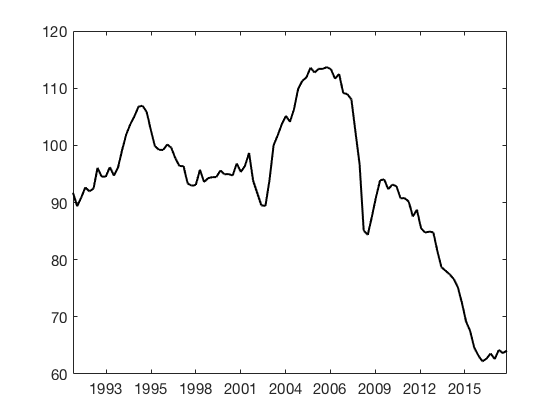
\includegraphics[width=\textwidth]{fig7}
        \caption{TCR}
    \end{subfigure}
    ~ %add desired spacing between images, e. g. ~, \quad, \qquad, \hfill etc. 
      %(or a blank line to force the subfigure onto a new line)
    \begin{subfigure}[b]{0.4\textwidth}
        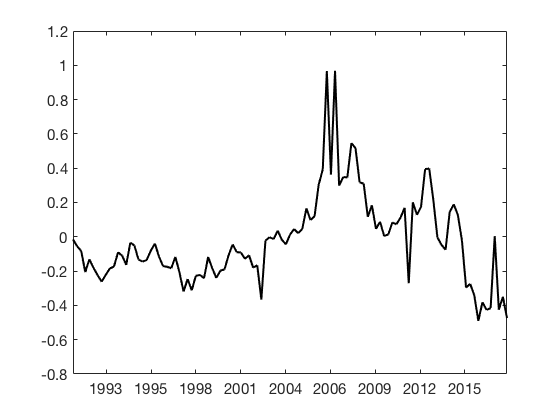
\includegraphics[width=\textwidth]{fig8}
        \caption{NFA}
    \end{subfigure}
    \begin{subfigure}[b]{0.4\textwidth}
        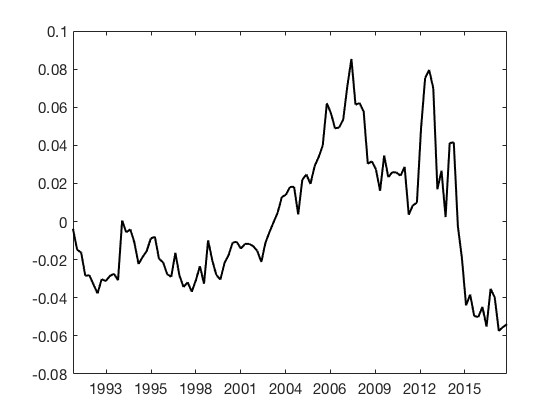
\includegraphics[width=\textwidth]{fig9}
        \caption{Saldo CC}
    \end{subfigure}
    ~ %add desired spacing between images, e. g. ~, \quad, \qquad, \hfill etc. 
    %(or a blank line to force the subfigure onto a new line)    
   \begin{subfigure}[b]{0.4\textwidth}
       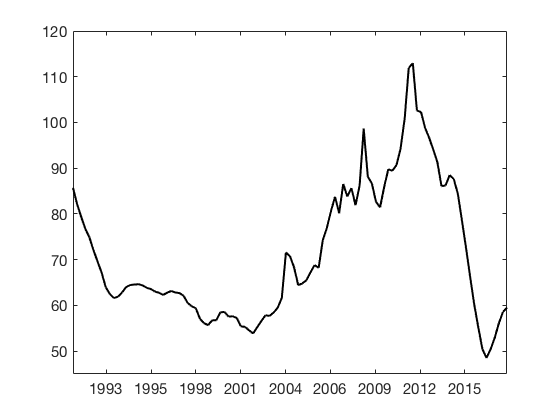
\includegraphics[width=\textwidth]{fig10}
        \caption{TI}
    \end{subfigure}
    \begin{subfigure}[b]{0.4\textwidth}
        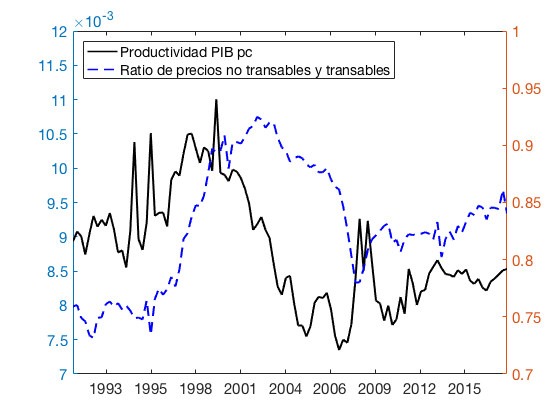
\includegraphics[width=\textwidth]{fig11}
        \caption{Productividad}
    \end{subfigure}
    ~ %add desired spacing between images, e. g. ~, \quad, \qquad, \hfill etc. 
      %(or a blank line to force the subfigure onto a new line)
    \begin{subfigure}[b]{0.4\textwidth}
        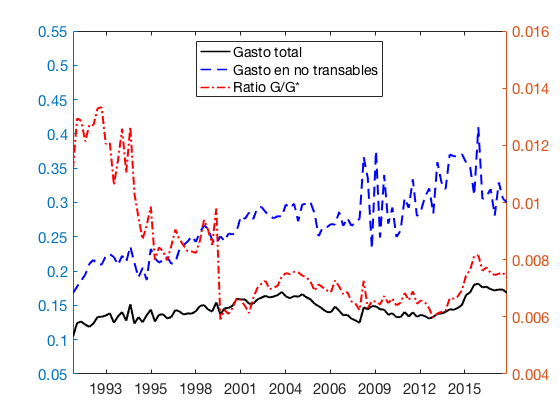
\includegraphics[width=\textwidth]{fig12}
        \caption{Gasto}
    \end{subfigure}
    \begin{subfigure}[b]{0.4\textwidth}
        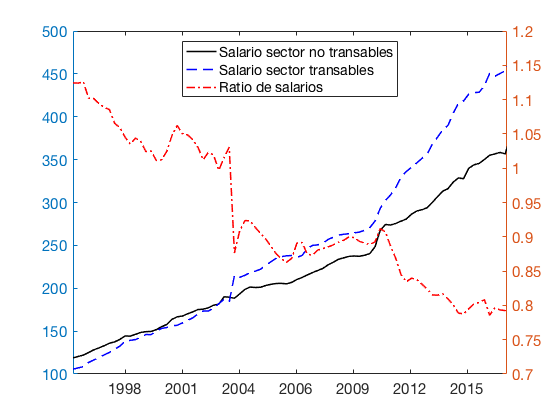
\includegraphics[width=\textwidth]{fig13}
        \caption{Salarios}
    \end{subfigure}
\end{figure}

Como ya ha sido mencionado, el tipo de cambio real y los términos de intercambio se los obtiene de las estadísticas publicadas por el Banco Central de Bolivia. La información tiene frecuencia trimestral, y en lo posible se la recopila para el periodo 1991-2017. Sin embargo, como se observa en los gráficos, la presencia del quiebre estructural en algunas variables previo a 2004, y en aras de obtener estimaciones robustas se realiza algunas de las estimaciones para el periodo 2004-2017.

Previo a realizar la estimación se efectúa un análisis de correlaciones cruzadas. El objetivo es documentar las principales regularidades de las variables escogidas como fundamentos con el TCR en el mediano plazo con el fin de entender la dinámica de equilibrio entre el bloque de variables a ser analizadas. En este sentido, se documenta la correlación máxima hallada para diez periodos de adelanto y de rezago. Este ejercicio junto con la dirección del rezago o adelanto ayudará a comprender los signos que se esperarían de la estimación, y permitirá evaluar el desempeño del modelo con la evidencia empírica.

En cuanto a metodología, las variables a ser analizadas son inicialmente desestacionalizadas con el filtro \emph{X-12 ARIMA}, a este conjunto de variables se les extrae el componente de mediano plazo con el filtro de alta frecuencia propuesto por \cite{christiano2003band}, la duración del periodo de estudio se asume entre 4 a 32 trimestres. Una vez removidos los componentes tendenciales se procede a calcular para cada par de variables (TCR y un fundamento a la vez) las funciones de correlación cruzada dinámica, los principales resultados se detallan a continuación:

\begin{itemize}
\item Con relación a las medidas de gasto, los tres indicadores reflejan que incrementos en el gasto de gobierno estarían asociados a una apreciación del TCR, la diferencia radica en el tiempo en el que cada variable alcanza su máxima correlación con el TCR. Por un lado, el gasto de gobierno en bienes no transables, tiende a adelantarse en un trimestre a los movimientos del TCR, es decir que presiones por parte del gobierno en los precios de los bienes no transables se traducirian en apreciaciones de TCR; por otro lado, la medida de gasto de gobierno total como proporción del PIB, tiende a moverse con rezago a las variaciones del TCR. 
En el caso del ratio que mide la relación gasto-pib domético con el foráneo, el indicador refleja que a medida que el gasto de gobierno crece más rápido en relación con el de sus socios comerciales se ejercerá presiones a los precios de los sectores, en este caso se asumiría que dicha presión es directa para el sector de bienes no transables por lo que el proceso de ajuste en los precios se reflejaría en una apreciación del TCR, no obstante al igual que en el caso previo la variable se rezagaría al comportamiento del TCR, lo que quizá evidencia el rezago, es que el ratio como tal no solo considera gasto en bienes no transables sino una medida de gasto total. 
\item Activos externos netos, la evidencia sugiere que esta variable en realidad se rezaga al comportamiento del TCR en al menos 9 trimestres, la dirección del comovimimiento señala que ante la disminución de pasivos externos netos se originarían presiones para la apreciación del TCR. Visto desde otro punto de vista una posición de activos externa más favorable, permitirá sostener en el tiempo la existencia de un défict fiscal que sería el resultado de mayor gasto en bienes no transables lo que llevaría a una apreciación. Por otro lado tambien se evidencia una correlación positiva a 1 periodo de rezago, que reflejaría a presiones en la depreciación, situación que sería coherente  si los precios no transables son mayores a los precios de productos transables y si los precios no transables externos son mayores a los precios de bienes no transables de Bolivia. 
\item Con relación a las medidas de productividad, se tienen conclusiones mixtas, el indicador que mide la productividad mediante la razón del PIB per cápita entre Bolivia y sus socios comerciales tiende a adelantarse a los movimientos del tipo de cambio real, la dirección de la correlación indica que aumentos en la productividad se asociarían a una apreciación del TCR. Mientras que un incremento de los precios de transables mayor al de los no transables provocaría una depreciación. Por su parte, el ratio de salarios no presenta una relación clara con el TCR.
\item Finalmente, según la literatura la relación de los términos con el tipo de cambio real puede ir en dos sentidos. Por un lado, puede dominar el efecto sustitución, es decir en un escenario en el que los bienes importados tienden a abaratarse con relación a los bienes exportados, se incrementaría la demanda por bienes importados, si los bienes son sustitutos su demanda caería los que presionaría una depreciación, este efecto según las funciones de correlaciones cruzadas se observaría a tres trimestres de rezago de los términos de intercambio con el tipo de cambio real con una correlación cercana al 50\%. El segundo canal podría darse a partir del efecto ingreso, según el cual existiría presión sobre el consumo de bienes no transables que se traduzcan en una apreciación del TCR, en la evidencia empírica esta relación reflejaría que los términos de intercambio preceden movimientos del tipo de cambio real con ocho trimestres de rezago y una correlación cercana al -30\%.
\end{itemize}

\begin{figure}
\captionsetup[subfigure]{aboveskip=-1pt,belowskip=-1pt}
\centering
\caption{Correlaciones}
\captionsetup[subfigure]{font=scriptsize,labelfont=scriptsize}
    \begin{subfigure}[b]{0.48\textwidth}
        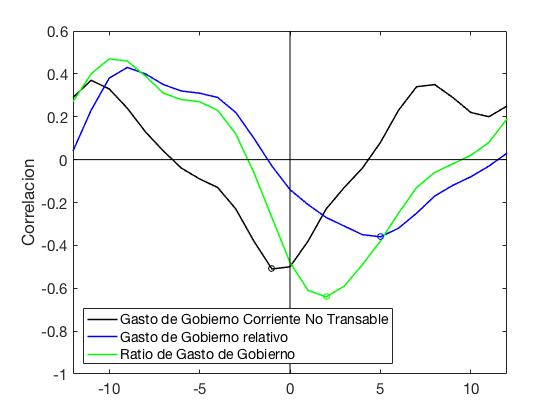
\includegraphics[width=\textwidth]{fig14}
    \end{subfigure}
    ~ %add desired spacing between images, e. g. ~, \quad, \qquad, \hfill etc. 
      %(or a blank line to force the subfigure onto a new line)
    \begin{subfigure}[b]{0.48\textwidth}
        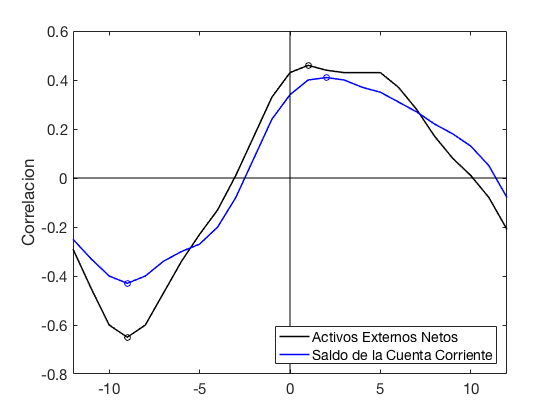
\includegraphics[width=\textwidth]{fig15}
    \end{subfigure}

    \begin{subfigure}[b]{0.48\textwidth}
        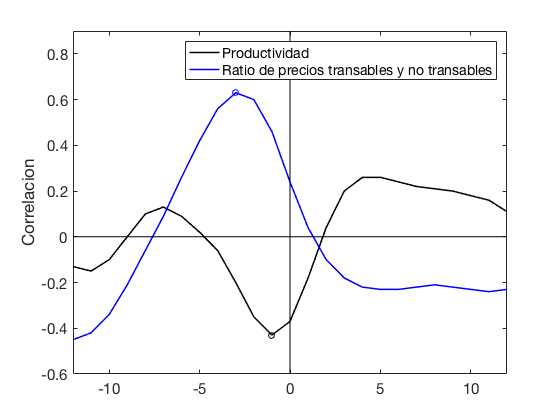
\includegraphics[width=\textwidth]{fig16}
    \end{subfigure}
    ~ %add desired spacing between images, e. g. ~, \quad, \qquad, \hfill etc. 
    %(or a blank line to force the subfigure onto a new line)
   \begin{subfigure}[b]{0.48\textwidth}
       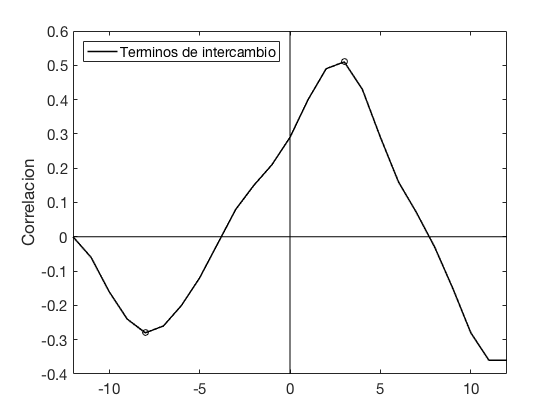
\includegraphics[width=\textwidth]{fig17}
    \end{subfigure}
  
   \begin{subfigure}[b]{0.48\textwidth}
       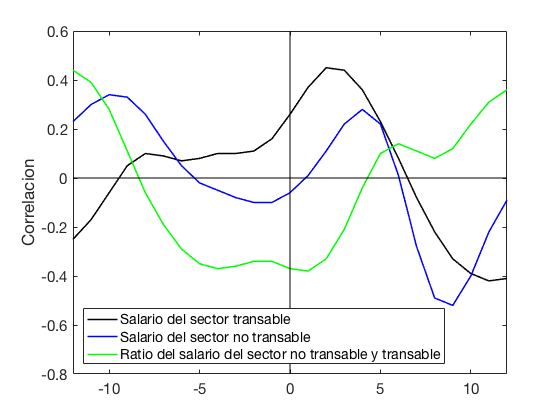
\includegraphics[width=\textwidth]{fig18}
    \end{subfigure}
\end{figure}

En el marco de la evidencia empírica descrita, se realiza la estimación mediante modelos de corrección de errores. Se presentan los resultados para tres especificaciones diferentes, Las más parsimoniosas serán los modelos 1 y 3. En el primer modelo los fundamentos serán el gasto de gobierno en bienes no transables como porcentaje del PIB, los activos externos netos como porcentaje del PIB, la relación entre precios transables y no transables y los términos de intercambio.

La medida de gasto de gobierno refleja las presiones hacia la apreciación en la medida en la que el valor tiende a incrementarse. Para el caso de los activos externos netos, la variable no tiene el signo esperado, lo que según la evidencia empírica descrita sería consistente con presiones a la depreciación toda vez que los precios de los bienes no transables serían mayores a los transables y los precios de no transables externos resultan mayores al de Bolivia lo que se traduciría en una presión a la depreciación. 

Con relación a las medidas de productividad, la relación de precios no transables y transables reflejaría el signo que se espera, es decir que un incremento del indicador se traduciría en una depreciación. Finalmente, los términos de intercambio reflejarían el efecto riqueza es decir presiones a la apreciación. 

El segundo modelo mantiene los signos esperados para el gasto de gobierno total, la productividad per capita y los términos de intercambio, mismas que generarían presiones a la apreciación según la descripción de la regularidades empiricas, por otro lado las variaciones en el ratio de la cuenta corriente con relación al producto, generaría presiones a la depreciación es decir mientras mayor sea el deficit en cuenta corriente no será posible cubrir un posible déficit fiscal y existiría una reducción en la demanda de bienes no transables generando presiones a la depreciación del TCR. 

A manera de ejercicio se realiza un modelo 2 con información desde 1996 hasta 2017 trimestre i, sin embargo como se menciono inicialmente el hecho de que en los años 90 se tuvieran todavia modificaciones estructurales en las variables no coadyuva en la estimación del modelo ya que las series terminan registrando mayor volatilidad y cuentan con propiedades menos favorables para su estimación. 

\begin{table}
\begin{center}
\caption{Modelos de cointegración}
\scalebox{0.8}{%
\begin{tabular}{lcccc}
\hline									
\hline									
	&	Modelo 1	&	Modelo 2 V1	&	Modelo 2 V2	&	Modelo 3	\\
Variable	&	ln(TCR)	&	ln(TCR)	&	ln(TCR)	&	ln(TCR)	\\
	&	1	&	1	&	0	&	1	\\
\hline									\\
Constante	&	4,239	&	3,323	&	-3,897	&	4,576	\\
ln(G_{NT}/Y)	&	-0,803	&	&	&	\\
	&	(0,138)	&		&		&		\\
ln(G/Y) &		&	0	&	-1	&	-1,580**	\\
	&		&		&		&	(0,321)	\\
AEN/Y	&	0,741**	&		&		&		\\
	&	(-7,428)	&		&		&		\\
CC/Y	&		&	6,172**	&	-1,106	&	7,236**	\\
	&		&	(0,650)	&	(0,253)	&	(1,035)	\\
ln(P_{NT}/P_T)	&	0,904**	&	0,554	&	0,452**	&		\\
	&	(0,128)	&	(0,327)	&	(0,127)	&		\\
ln(PIBpc/PIBpc^*)	&		&	-0,851**	&	-0,622**	&	-0,566	\\
	&		&	(0,233)	&	(0,091)	&	(0,374)	\\
ln(P_X/P_M)	&	-0,137*	&	-0,645	&	-0,207	&	-1,364*	\\
	&	(0,128)	&	(0,116)	&	(0,045)	&	(0,218)	\\
ln(W_{NT}/W_T)	&		&	0,622**	&	-0,005	&		\\
	&		&	(0,195)	&	(0,076)	&		\\
\hline							
\hline									
\end{tabular}%
}	
\end{center}
\begin{scriptsize}
\emph{Nota:} La significancia al uno, cinco y diez por ciento es indicad por ***, ** y *, respectivamente. El modelo 2 usa información trimestral desde 1996.I hasta 2017.I.
\end{scriptsize}								
\end{table}	

Vale la pena considerar que este tipo de modelos siempre presentará resultados que muestran que los datos observados parecen estar alrededor de la tendencia y dentro de las bandas de confianza del modelo. Esto porque básicamente el modelo de cointegración está usando los datos observados de tipo de cambio real y está calculando el modelo alrededor de ellos. Por tal motivo, no se verá divergencias grandes de la tendencia.

Sin embargo, lo particular de estos modelos son las variaciones que existen a un nivel de menor frecuencia, es decir los altos y bajos picos que puedan surgir que muestran el desequilibrio del modelo. Desde esa perspectiva y con relación a sus fundamentos, el tipo de cambio real se mantuvo en linea a sus fundamentos, destacan dos picos el primero al cierre de 2016 y el segundo durante 2011-2012, mientras que al cierre de 2016 e inicios de 2017 el valor del tipo de cambio real se encontraría por debajo de su valor de equilibrio.   

\begin{figure}
\centering
\caption{BEER}
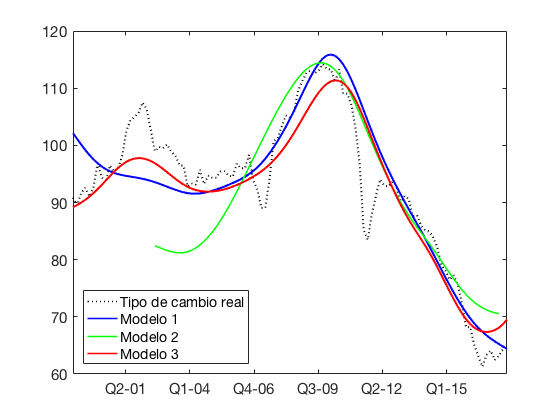
\includegraphics[scale=0.6]{fig19}
\end{figure}













\subsection*{FEER}

%datos
En primera instancia se realizan las estimaciones para las ecuaciones de comercio exterior. Lo que se busca es encontrar la elasticidad de exportaciones e importaciones en términos reales con respecto al tipo de cambio real y a la correspondiente medida de demanda de las mismas. Previamente, se verifican las propiedades individuales y en conjunto de las series en niveles. Nótese que todas las variables son integradas de grado 1 especialmente debido a la presencia de tendencias.

Las variables analizadas son: importación y exportación real (expresadas en moneda constante), PIB real de Bolivia (expresado en moneda constante), índice de los PIB de los principales socios comerciales de Bolivia, tipo de cambio real e índice de precios exportados por Bolivia. Mientras que el PIB, importaciones y exportaciones de Bolivia son de fuente Instituto Nacional de Estadística de Bolivia (INE)\footnote{Más adelante se utiliza los datos de la cuenta corriente boliviana, la misma que es fuente BCB. Hubiese sido ideal trabajar con las series de exportación e importación del BCB pues estas son las series utilizadas para calcular la cuenta corriente. Sin embargo, el cambio de metodología (al Manual de Balanza de Pagos 6, MBP6) bajo el cual se tienen calculados los años 2014, 2015 y 2016, hace imposible la concatenación de datos con los años pasados que están calculados bajo otras metodologías, por esta razón se opta por utilizar los respectivos datos con fuente del INE.}, las restantes variables son creadas y mantenidas por el \emph{BCB} (Banco Central de Bolivia). Todas las variables han sido desestacionalizadas por el métodos \emph{X-12 ARIMA}.

\begin{figure}
\centering
%\captionsetup[subfigure]{aboveskip=-2pt,belowskip=-2pt}
\caption{Variables incluidas en el modelo}\label{variables}
    \begin{subfigure}[b]{0.4\textwidth}
        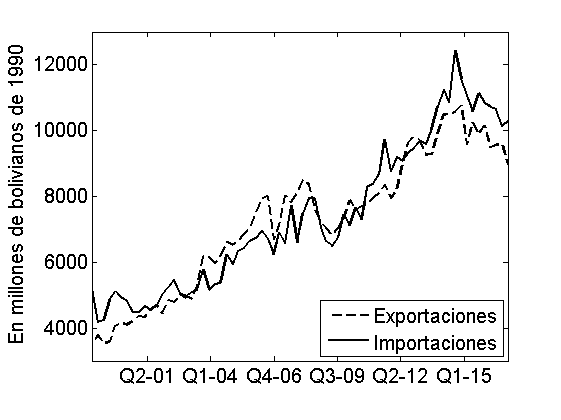
\includegraphics[width=\textwidth]{1xm}
        \caption{Exportación e importación}
        \label{1xm}
    \end{subfigure}
    ~ %add desired spacing between images, e. g. ~, \quad, \qquad, \hfill etc. 
      %(or a blank line to force the subfigure onto a new line)
    \begin{subfigure}[b]{0.4\textwidth}
        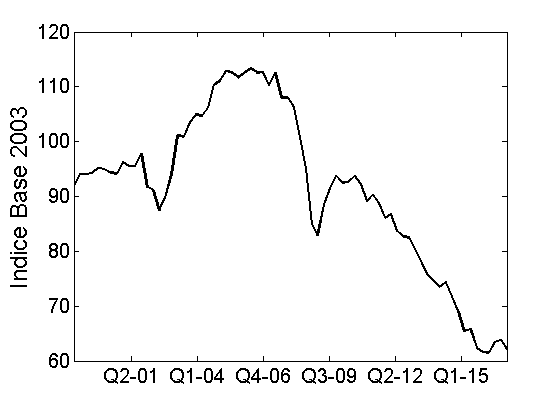
\includegraphics[width=\textwidth]{3tcr}
        \caption{TCR}
        \label{3tcr}
    \end{subfigure}
    \begin{subfigure}[b]{0.4\textwidth}
        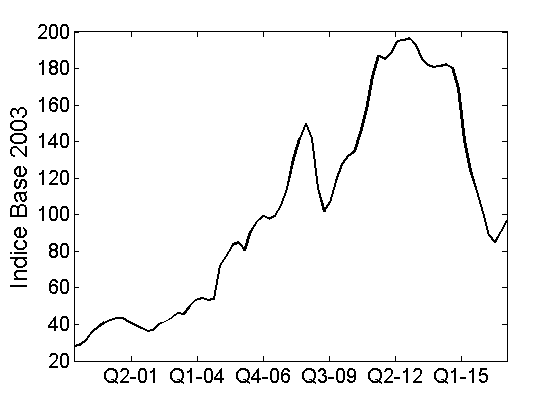
\includegraphics[width=\textwidth]{5ippbx}
        \caption{Precios internacionales}
        \label{5ippbx}
    \end{subfigure}
    ~ %add desired spacing between images, e. g. ~, \quad, \qquad, \hfill etc. 
      %(or a blank line to force the subfigure onto a new line)
    \begin{subfigure}[b]{0.4\textwidth}
        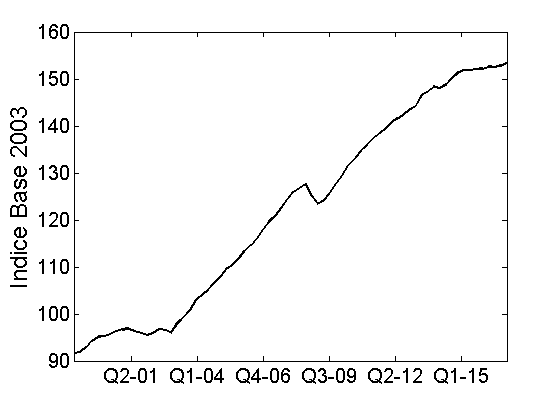
\includegraphics[width=\textwidth]{2per}
        \caption{PIB externo relevante}
        \label{2per}
    \end{subfigure}
    \begin{subfigure}[b]{0.4\textwidth}
        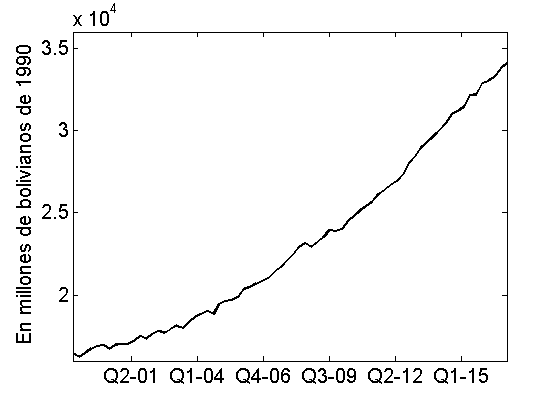
\includegraphics[width=\textwidth]{4pib}
        \caption{PIB}
        \label{4pib}
    \end{subfigure}
\end{figure}

En principio, la verificación gráfica sugiere que las series de importación y exportación comparten tendencia con el PIB de Bolivia y el índice de producto de sus principales socios comerciales, respectivamente. En el PIB boliviano se advierte una tendencia de crecimiento sostenido desde 1999, sin embargo, desde aproximadamente el 2009, esta presenta una aceleración que dura hasta 2013. El índice del PIB de los socios comerciales más importantes de Bolivia muestra una recesión en 2008 marcada por la crisis financiera internacional y un desaceleramiento a partir de 2013. Esta última variable parece reflejar mejor la tendencia del comercio internacional boliviano al compartir tendencia con las exportaciones. A pesar de que la serie del tipo de cambio real no parece presentar una relación en tendencia tan evidente como la señalada previamente, el índice de precios de productos bolivianos exportados parece compartir ciclos con la serie de exportaciones.

\begin{table}
\caption{Matriz de correlación}
\begin{center}
\begin{tabular}{lcccccc}									
\hline													
\hline												
	&	Exportaciones	&	Importaciones	&	PIB externo	&	TCR	&	IPPBX	&	PIB	\\
\hline													
Exportaciones	&	1	&		&		&		&		&		\\
Importaciones	&	0.9384	&	1	&		&		&		&		\\
PIB externo	&	0.9424	&	0.9751	&	1	&		&		&		\\
TCR	&	-0.5185	&	-0.7131	&	-0.7103	&	1	&		&		\\
IPPBX	&	0.8949	&	0.8506	&	0.8743	&	-0.3589	&	1	&		\\
PIB	&	0.9017	&	0.9645	&	0.9835	&	-0.8102	&	0.7821	&	1	\\
\hline													
\hline									
\end{tabular}	
\end{center}						
\begin{scriptsize}
\emph{Nota:} Elaboración propia.
\end{scriptsize}	
\label{corre}	
\end{table}	

Para verificar el análisis gráfico se calcula la matriz de correlación de las variables previamente señaladas, las cuales se muestran en la tabla \ref{corre}. Como había sido adelantado, el PIB externo relevante es la variable más fuertemente asociada a las exportaciones e importaciones seguidas por PIB boliviano y el índice de precios de exportaciones que, como era de esperar, está más correlacionado con las exportaciones. Por otro lado, el tipo de cambio real presenta una correlación negativa con ambas variables especialmente con las importaciones. Bajo este adelanto parece ser que los signos propuestos en la ecuación \ref{M} se cumplirían mientras que en la ecuación \ref{X} el TCR presentaria el signo contrario al esperado.

\begin{table}
\caption{Regresiones de Comercio}
\begin{center}
\scalebox{0.8}{%
\begin{tabular}{lcccc}									
\hline									
\hline	
	&	(1)	&	(2)	&	(3)	&	(4)	\\
	&	$X$	&	$\Delta x$	& $M$	&	$\Delta m$	\\
\hline	
$y^*$	&	1.700***	&		&		&		\\
	&	(0.035)	&		&		&		\\
$\Delta y^*$	&		&	1.135*	&		&		\\
	&		&	(0.626)	&		&		\\
$y$	&		&		&	1.008***	&		\\
	&		&		&	(0.020)	&		\\
$\Delta y$	&		&		&		&	1.018	\\
	&		&		&		&	(0.353)	\\
$tcr$	&	0.155***	&	&	-0.276***	&	\\
	&	(0.037)	&	&	(0.044)	&	\\
$\Delta tcr$	&	&	0.499**	&	&	-0.095	\\
	&	&	(0.212)	&	&	(0.075)	\\
\hline									
\hline									
\end{tabular}%
}
\end{center}
\begin{scriptsize}
\emph{Nota:} La significancia al uno, cinco y diez por ciento es indicada por ***, ** y *, respectivamente.
\end{scriptsize}								
\label{Rec}	
\end{table}	

En el cuadro \ref{Rec} se resume los resultados de las regresiones de comercio en las que las correspondientes variables se encuentran logaritmizadas. Se ensayan dos regresiones lineares por cada componente, primero en niveles y después en diferencias. Los resultados en niveles representan las relaciones de largo plazo por entenderse que comparten que las series de comercio comparten tendencia con sus correspondientes demandas. Por otro lado, los resultados en diferencias corresponden a las relaciones de corto plazo. Por tanto, se podría utilizar los resultados de elasticidades que convengan.

En primer lugar, se debe aclarar que el cuadro \ref{Rec} evidencia que las relaciones de largo plazo son mucho más significativas. Efectivamente, este resultado deriva de que definitivamente comparten tendencias que son responsables de la dirección de las realizaciones de las variables dependientes. A pesar que las regresiones de corto plazo no son tan significativas, la interpretación de este resultado es muy importante. 

Las variables de comercio se muestran especialmente inelásticas a las realizaciones del TCR. Los resultados muestran que en el comercio depende de las tendencias de sus demandas y son significativamente insensibles a la tendencia del TCR a pesar de reproducir los signos esperados. Los componentes cíclicos, es decir las variaciones alrededor de la tendencia, no tienen efecto en las importaciones, mientras que las exportaciones muestran inelasticidad significativa.

Esto se traduce en la ineslasticidad del comercio al TCR en el largo plazo, pero aún así la tendencia en la que esta última variable se mueve tiene influencia, en especial, en las importaciones. En contraste, en el corto plazo las importaciones parecen no tener sensibilidad alguna al TCR, pero las importaciones si aunque bastante inelásticamente. Asimismo, parece ser que existen otros factores como términos de intercambio y precios que podrían determinar las variaciones a corto plazo de las series de comercio. Sin embargo, se muestra una significancia importante en la elasticidad del comercio a las demandas especialmente en el corto plazo a pesar de perder significancia en el corto plazo.

\begin{figure}
\captionsetup[subfigure]{aboveskip=-2pt,belowskip=-2pt}
\centering
\caption{Estructura de importaciones y exportaciones de Bolivia}\label{impexp}
    \begin{subfigure}[h]{0.65\textwidth}
        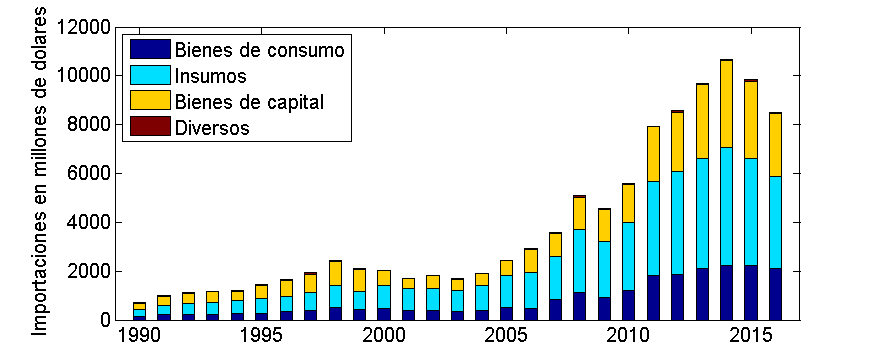
\includegraphics[width=\textwidth]{imp9016}
        \caption{Estructura de importaciones}
        \label{mestr}
    \end{subfigure}
    \begin{subfigure}[h]{0.65\textwidth}
        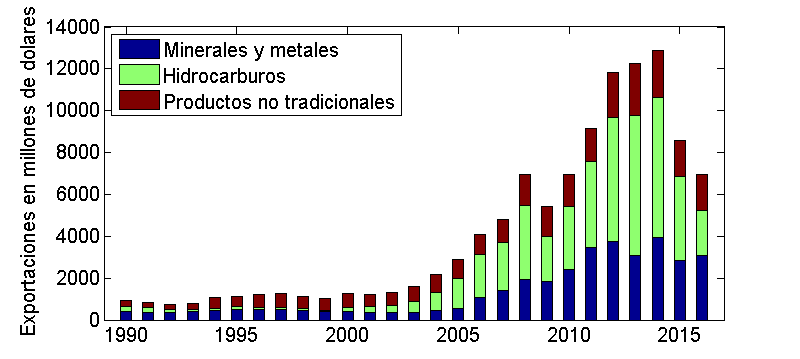
\includegraphics[width=\textwidth]{exp9016}
        \caption{Estructura de exportaciones}
        \label{xestr}
    \end{subfigure}
\end{figure}

Nótese en el gráfico el gráfico \ref{3tcr} que el TCR se aprecia sostenidamente entre 2007-2016.\footnote{Obviando el quiebre que sucedió durante la crisis financiera internacional que al final no afecto a la tendencia del comportamiento del TCR.} Este comportamiento, contrastado a los gráficos \ref{1xm}, coincide con el crecimiento sustancial de las exportaciones e importaciones. Mientras que la teoría indica que una apreciación de estas características debería haber afectado negativamente a las exportaciones y positivamente a las importaciones. Pero como se puede ver en el gráfico \ref{xestr} la apreciación real favoreció positivamente incluso a los bienes no tradicionales en los cuales destaca soya y sus derivados, madera, joyería, castaña y otros productos menos frecuentes.

La explicación de este fenómeno es interesante y depende de las características particulares del comercio externo boliviano. Las exportaciones bolivianas de hidrocarburos y minerales representan, en promedio, el 78\%, desde la nacionalización de hidrocarburos en Bolivia en 2006 y alcanzando los niveles más elevados de representación entre 2011-2014. Los precios de estos productos tradicionales están definidos en los mercados internacionales; donde la limitada oferta boliviana no tiene influencia en la determinación del precio internacional. Las materias primas, al tener el mismo precio en todos los países generalmente en dólares, no son medidas por el tipo de cambio real y tampoco influencias por ellas pues dicha medida no las incluye.\footnote{Recuérdese que el TCR es construido con índices de precios al consumidor en los que las materias primas no entran en la canasta de ningún país.} A priori se estima que por construcción esta variable solo tendría una influencia con la exportación de bienes no tradicionales o manufacturas, las cuales tienen una participación mucho menor en las exportaciones totales, en especial si se la compara, por ejemplo, con el gas y los minerales exportados. Las manufacturas oscilan en participación entre 12-25\% entre 1999 y 2006 y 7-12\% en 2007-2016 siendo este último periodo en el que el volumen exportado de manufacturas se llegó a multiplicar por lo menos por tres. Finalmente, nótese que las exportaciones no tradicionales que destacan en su crecimiento no corresponden en todos los casos a bienes finales, sino la mayoría constituyen bienes intermedios cuya competitividad externa no es medida en el TCR.

Por el lado de las importaciones, la estructura no es tan variable a través de los años a pesar del incremento notable suscitado en 2004 y confirmado en 2005. La pregunta es: porqué la marcada correlación positiva de crecimiento y apreciación no generaron elasticidades positivas de TCR en los modelos del cuadro \ref{Rec}. La respuesta es porque prima el efecto ingreso, eso quiere decir que sin importar el encarecimiento relativo de los bienes extranjeros, el incremento del ingreso nacional impulsó la demanda de importaciones fuertemente. Es por este motivo que se registra una alta elasticidad con respecto a la demanda caracterizada por el PIB local. Además, nótese que Bolivia importa una gran cantidad de insumos y bienes de capital que no son representados por el TCR. Alternativamente, se ejercita una variedad de explicaciones por las cuales la ineslasticidad demanda-precio de la serie sin tendencia en importaciones es tan marcado al grado de no ser significativa ni siquiera en bajos niveles.

\begin{itemize}
\item La pequeña industria boliviana no alcanza para satisfacer la demanda boliviana de bienes por lo que las importaciones son precio inelásticas. Al mismo tiempo, no existen productos domésticos para sustituir a las importaciones.
\item El precio de los bienes bolivianos es muy elevado, por lo que se prefieren los precios más bajos importados incluso frente a un tipo de cambio muy devaluado. Esto podría ser ocasionado por el uso de tecnologías domésticas atrasadas o caducas que hacen que los precios domésticos sean más elevados incluso con salarios bajos.
\item La calidad de los bienes importados es superior a la producción doméstica. Esto podría deberse a que la tecnología doméstica es atrasada o que el costo de producir mayor calidad es muy elevado. Por otro lado, relacionando esta hipótesis con la previa se puede pensar que el precio doméstico no es acorde a la calidad ofrecida por lo que la demanda de bienes importados es inelástica al tipo de cambio real. 
\end{itemize}

De todas maneras, del Cuadro \ref{Rec} se rescata que el comercio externo es muy sensible al rendimiento de las economías extranjeras, y en el caso de las importaciones al de la economía doméstica. La baja sensibilidad al tipo de cambio real implica que sería necesario cambios muy elevados de este para generar variaciones significativas en el comercio externo boliviano. Las elasticidades estimadas son utilizadas para calcular el tipo de cambio real de equilibrio, en el que se utilizan los valores tendenciales de demanda doméstica, demanda externa y precios de exportaciones.

Posteriormente se estima la varianza de la variación estimada y se hace la medición para encontrar el valor de equilibrio del tipo de cambio real.

\begin{figure}
%\captionsetup[subfigure]{aboveskip=-2pt,belowskip=-2pt}
\caption{Resultados DEER}
\centering
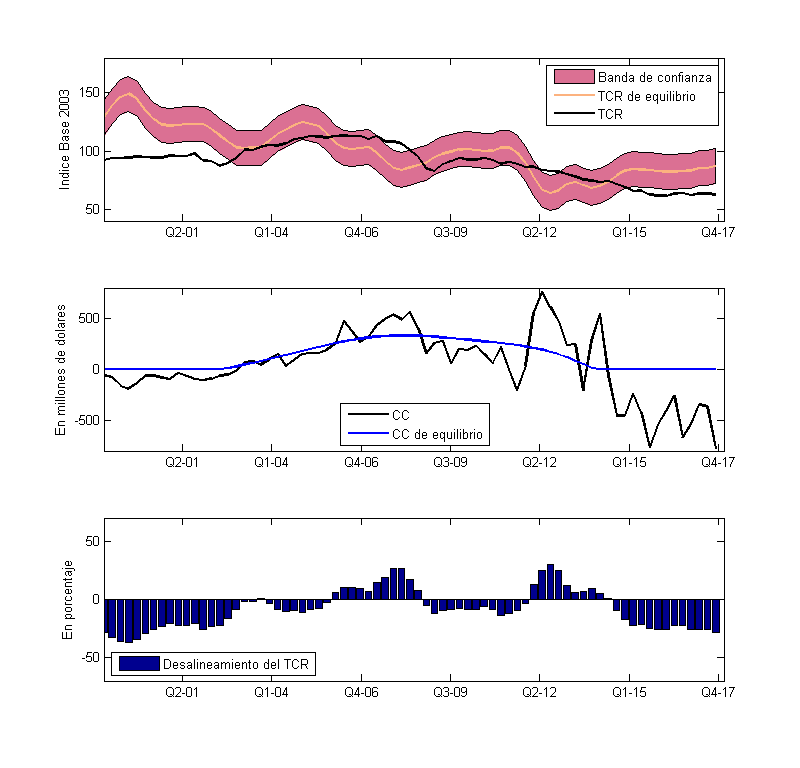
\includegraphics[scale=0.7]{tcreq}
\end{figure}

De esta evidencia se verifica que el tipo de cambio real estuvo desalineado durante dos periodos de la muestra planteada. A partir del 2006 la diferencia entre el tipo de cambio real observado y de equilibrio tiende a ser mucho menor. A partir del 2014 la divergencia de ambas series comienza a ser fuerte. En estos periodos de desequilibrio se entiende que el tipo de cambio real se encontraba sobre valuado. Es decir que para restaurar el equilibrio era necesario devaluar el boliviano. En efecto, si verificamos paralelamente a los tipos de cambio reales observados y de equilibrio junto con la cuenta corriente observada y de objetivo podemos verificar que los desalineamientos en tipo de cambio coinciden con los de cuenta corriente. 

Desde esta óptica, es importante verificar que la mayor variación de cuenta corriente correspondiente a 2013 y la tendencia a la baja ya eran indicios importantes para que gestionar la política que pueda generar la depreciación del tipo de cambio real para poder conseguir el equilibrio externo y evitar los déficits incurridos.

Es importante notar que las variaciones de tipo de cambio son un tema particularmente delicado en Bolivia por la historia inflacionaria y el hecho que la economía está anclada nominalmente al valor del dólar. Por otro lado, al ser las exportaciones dependientes del precio de las materias primas que comercia internacionalmente un buen indicador de la dirección que la balanza comercial, y por ende, la cuenta corriente vayan a tomar son los precios de materias primas exportadas. Ceteris paribus se puede calcular cual es la medida en la que el tipo de cambio nominal debería ser depreciado para mantener un equilibrio con cuenta corriente no deficitaria.

Otro punto interesante de estos resultados se enfoca en el periodo previo a 2006. El mismo implica que durante la época neo liberal el tipo de cambio real no estuvo alineado con sus valores de equilibrio a pesar de depreciar el tipo de cambio nominal en función al tipo de cambio referencial que supuestamente  mantiene el tipo de cambio real constante y competitivo. Por lo menos, la cuenta corriente y balanza comercial se encontraron en déficit sostenidos, lo cual bajo ningún concepto se traducen a niveles de equilibrio de tipo de cambio.

%\footnote{Si bien esto es cierto, en la realidad los bienes primarios transados bilateralmente entre países tienen como precio aplicable aquel pactado en los contratos suscritos entre partes, el cual puede ser o no el mismo que los determinados por los mercados internacionales, tal vez debido a otros factores como la calidad o el costo de transporte u otras consideraciones. Sin embargo, y sin lugar a dudas estos precios internacionales son el referente de los precios últimos contratados por materias primas.}	






\section{Consideraciones Preliminares}\label{consid}


%\subsection*{Movimientos del tipo de cambio real}
Debido a que la fórmula de tipo de cambio real es la definida por \ref{tcr1} o \ref{tcrlog} y el tipo de cambio nominal es el principal instrumento de la política cambiaria, se hace tentador simplemente despejar esta variable de la fórmula para que ella indique cual, para el nivel deseado de tipo de cambio real, es el nivel de depreciación nominal necesario para lograr el nivel de TCR definido. Este es el método mediante el cual se encuentra el tipo de cambio referencial al que se hace mención en la introducción de este documento. Sin embargo, el uso de esta estrategia puede ser considerado una falacia teórica.

La razón es porque, en contraposición de los precios extranjeros que son exógenos, los precios de la economía doméstica dependen, o están en función entre otras cosas, del tipo de cambio nominal $p(e)$. Al respecto, la evidencia más grande está en la literatura de \emph{pass-through} de tipo de cambio a inflación, la cuál generalmente obtiene valores distintos de cero y positivos. El hecho que el coeficiente de \emph{pass-through} sea distinto de cero implica que la depreciación del tipo de cambio nominal, desde una perspectiva de instrumento, genera presiones en el nivel de precios hacia el alza. Entonces, tanto el tipo de cambio nominal como el nivel de precios se incrementan determinando que en el corto plazo el efecto de una devaluación nominal se aminore.

En la realidad existen dos factores empíricos importantes que matizan esta situación. El efecto \emph{pass-through} no se da inmediatamente debido a la rigidez de precios, es decir que la transmisión del incremento del tipo de cambio a los precios no ocurre inmediatamente sino a medida que los precios se reajustan a dicho cambio, únicamente una economía con total flexibilidad de precios o indexada perfectamente a la divisa de referencia transmitiría inmediatamente dicho efecto. Por otro lado, es un caso muy extremo cuando el parámetro \emph{pass-through} llegue a ser unitario pues implicaría que no solamente el sector transable es perfectamente sensible sino también el sector no transable lo es, en cuyo caso se podría pensar que el tipo de cambio afecta a los costos importados de bienes no transables. Otra probable explicación es que el efecto en los precios transables y no transables sobre-reaccionen debido a las expectativas inflacionarias y/o devaluativas haciendo que el efecto total de \emph{pass-through} llegue a la unidad, lo cual implicaría que la economía se encuentra en una posición demasiado riesgosa.

Otra consideración importante es que el nivel de \emph{pass-through} es variable, es decir que no es fijo a través del tiempo si no que depende de la situación particular en el que cada economía esté. Esto probablemente debido a la formación de las expectativas de los agentes. Por tanto, el uso adecuado del tipo de cambio nominal es complicado y sensible a varias consideraciones.

En el caso de Bolivia, el uso de la regla cambiaria siguiendo el tipo de cambio de referecia, es decir  utilizando la estrategia previamente mencionada, mientras estuvo vigente el \emph{crawling peg} no se logró la fijación del tipo de cambio real en el valor deseado. Durante el periodo en el que este régimen estuvo vigente el tipo de cambio real se situó volátilmente bajo su meta y durante 1994 y 1995 por encima de ella, mientras que la constante depreciación buscaba y suponía lograr el valor deseado puntualmente en cada periodo.

En realidad, lo que demuestra el comportamiento durante 1990 y 2003 es que la velocidad de la depreciación es menor que el de los precios internos dado el ajuste al nivel de precios externos exógenos. Potencialmente, esto implicaría que la aceleración de la depreciación generaría una velocidad aún mayor en el nivel de precios local. Esto implica que no se logra tomar en cuenta el efecto inflacionario de la devaluación en el nivel de precios locales. En particular, el desajuste entre 1994 y 1995 se debe principalmente al repunte inflacionario de Brasil, uno de los principales socios comerciales de Bolivia que en estas fechas introduce el real como moneda oficial, este factor externo originó que la moneda boliviana se deprecie más de lo esperado en términos reales. Al mismo tiempo, este evento se constituye en un shock que marca la leve desaceleración de la depreciación boliviana que no es tan pronunciada como la sugerida por su tipo de cambio referencial.

Es posible que la moderada depreciación y el anclaje de la expectativas de los agentes en la misma depreciación colaboró a que la inflación importada de Bolivia no sea incluso más elevada. Sin embargo, este hecho demuestra empíricamente la falacia teórica acerca de como mover el tipo de cambio real con su parte nominal.











\section*{Conclusiones}\label{concl}

Los modelos muestran que bajo el objetivo de sostenibilidad externa utilizado los mayores desajustes corresponden a los periodos en los que la cuenta corriente se encuentra en desequilibrio principalmente por los déficits en balanza comercial. Al mismo tiempo, estos periodos coinciden con aquellos en los que los precios de materias primas no fueron lo suficientemente beneficiosos para el esquema comercial internacional boliviano.

A pesar de que hasta 2004 se siguió una regla cambiaria que buscaba determinar al tipo de cambio real en un nivel fijo de competitividad, la evidencia muestra que esta política falló fuertemente, pues no consideró que al depreciar el tipo de cambio nominal, este se contrarrestaría con el movimiento de la inflación determinado por el efecto \emph{pass-through}, este es sólo uno de los motivos por los que esta regla cambiaria no funcionó para conservar un nivel estable de tipo de cambio real, Rodrik menciona otro, la falta de capacidad para generar ilusión monetaria. Al mismo tiempo, las mini-devaluaciones solamente sirvieron para ayudar un pequeño grupo de exportadores de manufacturas, mientras que hacía que las importaciones se encarecieran constantemente en términos de la moneda boliviana, esta es la raiz de una sostenida inflación importada y de la dolarización de ese periodo debido a que las expectativas cambiarias de la población estaban ancladas en la depreciación.

Durante el boom de los precios de materias primas y muy en especial después de la nacionalización de hidrocarburos en Bolivia el 2006 se vivió el recuperamiento de la balanza comercial dado que la mayoria de las exportaciones eran el gas vendido a Brasil y Argentina. Este hecho representó una gran entrada de divisas a la economía que fortaleció a las RIN y dotó de suficientes dólares americanos para cubrir los requerimientos de los mismos en el mercado interno. La apreciación real de la moneda significó que en este periodo de auge económico sea conveniente importar bienes. Por otro lado, el ancla nominal cambiaria se fijó en la estabilidad del boliviano. Este hecho contribuyó a la des-dolarización de la economía.

Finalmente, después de la caída de precios internacionales de materias primas, la economía boliviana logró sobrevivir por la solidez ganada en periodos previos y los aún significativos ingresos de hidrocarburos. Sin embargo, la cuenta corriente se vio afectada así como las RIN. Si bien durante este periodo la opinión pública reclamó una depreciación se considera que por la evidencia expuesta previamente, esta medida no podría haber podido cumplir el fin deseado de nivelar de nuevo la balanza comercial debido a que el volumen de la exportación de gas y minerales no dependen de esta variable.

Como se ha visto, la estabilidad cambiaria tiene gran aporte en la des-dolarización de la economía, sin embargo, el gobierno boliviano no ha delusidado aún la manera de mantener un tipo de cambio real estable y la evidencia señala que aún está experimentando con los instrumentos que tiene a su disposición. Asimismo, el auge económico respaldado por el comercio internacional fue patrocinado por el incremento de los precios del gas que también coincidió con la apreciación del tipo de cambio real y la débil consecución de la regla cambiaria que posteriormente fue abandonada al encontrar en en la estabilidad un refugio para permitir que la moneda local se fortalezca en el mercado interno que fue beneficiado por bajos precios de importaciones que a su vez beneficiaron a la mayor parte de la población que se dedica a este rubro y que a su vez permitió el crecimiento del sector no transable del país.


Como se ha evidenciado, el tipo de cambio real no es muy influyente para mover la balanza comercial debido a la inelasticidad de sus componentes a esta variable. Sin embargo, se han determinado los periodos en los que, dada la situacón y si el tipo de cambio fuese más flexible, el movimiento del tipo de cambio hubiese mejorado la situación de la economía.

%La regla cambiaria utilizada es incorrecta porque no determina la dirección del TCR, este punto ya ha sido probado hace tiempo.

%Bolivia necesita entre otras cosas una industria que produzca transables y no transables sustituibles dentro de la economía y fuera también, sin eso estamos dependiendo fuertemente de los designios de los movimientos de la economía extranjera.

En esa línea, la segunda metodología permitió establecer los fundamentos que se asocian al tipo de cambio real de equilibrio, los más consistentes fueron el gasto de gobierno, los términos de intercambio, los activos externos netos y la relación de precios transables y no transables. Este análisis permitió identificar que según la evidencia empírica por lo general los fundamentos tienden a anticipar los movimientos del tipo de cambio real, en esa línea el gasto de gobierno y las medidas de productividad mantienen la relación que se espera, mientras que los términos de intercambio transmitirían un efecto riqueza y no uno de sustitución. Si bien según la metodología se espera que el valor del tipo de cambio real se mantenga alineado se constan quiebres específicos, asociados a factores internos y externos, en los que se observan desalineamientos, sin embargo en términos generales el Tipo de cambio real se mantiene en línea con la evolución de sus fundamentos. 

%Posibilidad de enfermedad holandesa. no existe porque no hay otro sector que se pueda matar.


%Hay que entender que el tipo de cambio real está calculado en base a las variaciones de los índices de precios al consumidor de los socios comerciales y local y de los tipos de cambio. Como se toma en cuenta los índices de precios al consumidor, esta medida captura la variación real de artículos que entran en la canasta básica de consumo de cada país. Es evidente que esta puede diferir entre economías, sin embargo, el cálculo del tipo de cambio real hace abstracción de estas divergencias y asume que son lo suficientemente parecidas. El punto importante que se debe notar es que captura los precios de bienes de consumo interno y que están dentro de la canasta básica, los cuales no son bienes que Bolivia exporta, en contraposición si son bienes que importa. Por este motivo es que la inclusión de los valores 


\bibliographystyle{apalike}
\bibliography{tcr_bolivia}
\end{document}
